\chapter{Межпроцедурный анализ на основе резюме для метода символьного выполнения} \label{chapt2}

Для использования в разрабатываемой системе был выбран метод межпроцедурного анализа с использованием резюме.
Это связано с такими преимуществами метода, как повторное использование результатов анализа функции и возможностью выбора степени детализированности анализа. Схема межпроцедурного анализа с использованием резюме представлена на рис.~\ref{pic:summary-idef0-ll}.

\begin{figure}
   \centering
   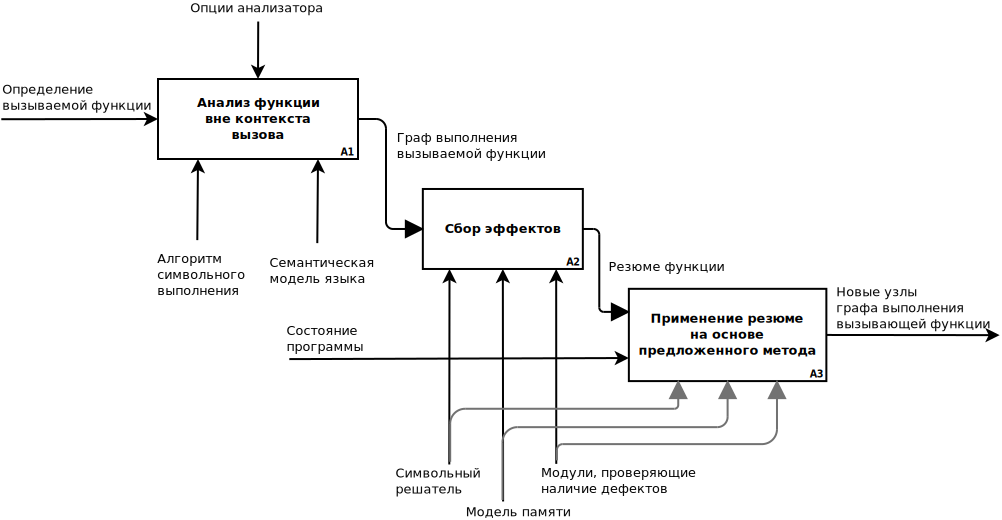
\includegraphics[width=\linewidth]{summary-idef0-ll.pdf}
   \caption{Метод межпроцедурного анализа с использованием резюме}\label{pic:summary-idef0-ll}
\end{figure}


\section{Математическая модель. Разработанный алгоритм метода резюме для символьного выполнения}

Рассмотрим основные источники затрат при~встраивании и~при использовании резюме. При~встраивании функций вызываемая функция анализируется каждый раз при~её вызове. При~этом в~случае контекстно-чувствительного анализа функция анализируется не~полностью: анализируются лишь те пути выполнения, которые являются достижимыми при~контексте на~момент вызова. Суммарное время, затраченное на~анализ функции при~допустимой степени вложенности, равной 1, можно вычислить по формуле:

\begin{equation}
 T_{\text{встраивания}} = \sum_{i = 0}^{n} t_i 
\end{equation}

где $i$ — номер вызова, $t_i$ — время, затраченное на~анализ $i$-го вызова (с~учётом контекста). С~учётом того, что сама вызываемая функция также анализируется отдельно, формула приобретает вид:

\begin{equation}
 T_{\text{встраивания полное}} = T_{\text{анализа}} + \sum_{i = 0}^{n} t_i 
\end{equation}

При~использовании подхода, основанного на~резюме, временные затраты вычисляются следующим образом. Вызываемая функция анализируется один раз, но полностью (независимо от~вида анализа). Однократный характер также носят затраты, связанные с~составлением резюме функции. Применение резюме выполняется в~каждой точке вызова функции. Таким образом, общие затраты рассчитываются по формуле:

\begin{equation}
 T_{\text{резюме}} = T_{\text{анализа}} + T_{\text{сбора}} + \sum_{i = 0}^{n} t_{i \text{применения}}
\end{equation}

что, с~учётом примерного равенства времён применения резюме (поскольку резюме имеет не~меняющийся размер), приближённо равно


\begin{equation}
 T_{\text{резюме}} = T_{\text{анализа}} + T_{\text{сбора}} + n t_{i \text{применения}}
\end{equation}

Таким образом, выигрыш от~применения резюме будет получен при~выполнении следующего соотношения:

\begin{equation}
 T_{\text{сбора}} + n t_{i \text{применения}} < \sum_{i = 0}^{n} t_{i}
\end{equation}

откуда следует, что для~получения ускорения необходимо выполнение соотношения

\begin{equation}
 t_{\text{ср. применения}} <  t_{\text{ср.}}
\end{equation}

Рассмотрим процесс анализа выполнения программы как систему состояний и переходов с ограниченной обозримостью.


Пусть $o_1, \ldots, o_n$~--- некоторая последовательность операторов программы. Каждый оператор программы представляет собой передаточную функцию: $s_i = o_i(s_{i-1})$, где $s_{i-1}$~--- состояние программы непосредственно перед выполнением оператора, $s_i$~--- состояние программы непосредственно после выполнением оператора  $o_i$ (и перед выполнением оператора $o_{i+1}$). Данная запись позволяет определить неформально \textit{эффект} оператора или последовательности операторов программы как различие между состояниями программы до и после выполнения оператора (формальное определение приводено далее). Тогда в~результате выполнения всего блока операторов программа из начального состояния $s_0$ перейдёт в~состояние $s_n$: $s_n = o_n(o_{n-1}( \ldots o_i( \ldots (o_1(s_0)) \ldots ))$. Тогда суммарный эффект последовательности операторов можно представить в~виде композиции их передаточных функций:
\begin{equation}
 o = o_1 \circ o_2 \circ \ldots \circ o_n
\end{equation}


Данная формула справедлива для~последовательности операторов без переходов, то есть для~базовых блоков программы. Кроме того, формула справедлива для~последовательности операторов, содержащей безусловный переход, поскольку такая последовательность также представляет собой путь выполнения без ветвлений. Однако при~наличии условных переходов в~блоке последовательности операторов, оказывающих эффект на~выполнение программы, могут различаться. Это означает, что суммарный эффект выполнения блока зависит от~пути выполнения внутри блока, а~следовательно, и~от значения  выражения в~условии.

Пусть $c_j$~--- условие, принадлежащее анализируемому блоку, $0 \leqslant j \leqslant m$, в~ветках \texttt{if} и~\texttt{else} которого находятся непрерывные последовательности операторов $o_0, \ldots, o_k$ и~$o_{k+1}, \ldots, o_n$ соответственно, возможно, пустые. Тогда будет справедливо следующее соотношение:

\begin{equation}
    s_c  =
     \left\{
    \begin{matrix}
    o_1 \circ \ldots \circ o_k & \text{при } c_j \equiv true \\
    o_{k+1} \circ \ldots \circ o_n & \text{при } c_j \equiv false
    \end{matrix} \right.
\end{equation}

С~использованием данных правил можно строить композиции эффектов произвольных последовательностей операторов.

Поскольку тело функции также является последовательностью операторов языка, эффект от~вызова функции можно рассчитать по тем же правилам. На~основе зависимости полученного эффекта от~условий на~пути выполнения внутри функции и~строится резюме. При~этом в~резюме сохраняются не~все эффекты, производимые операторами, содержащимися в~теле функции, а~лишь те из них, которые сохраняются после выхода из неё и~могут повлиять на~дальнейшее выполнение программы после выхода из функции. Таким образом, сократить время анализа при~использовании резюме в~сравнении со~встраиванием можно получить за~счёт отсутствия необходимости затрачивать время на~анализ эффектов, действия которых локальны или не~учитываются при~дальнейшем анализе. Так, связывание символьного значения с~выражением имеет только локальный эффект, поскольку все выражения становятся неактивными при~выходе из контекста анализа функции. Аналогично, локальный эффект имеют записи в~локально видимую память и~т.~д. Кроме того, модель анализатора заведомо допускает упрощения, поскольку анализатор не~может досконально смоделировать поведение программы. Это означает, что~ряд эффектов операторов не~будет учтён, т.~е. на~моделирование некоторых эффектов операторов будет затрачено время, однако результат этого моделирования не~будет отражён в~изменении состояния. Учёт этих упрощений и~ограничений анализатора позволяет устранить непроизводительные затраты времени, поскольку при~применении резюме непроизводительные вычисления не~выполняются повторно. Возможно, однако, что~некоторые эффекты самого применения резюме не~могут быть учтены моделью анализатора и~также будут отнесены к~непроизводительным вычислениям. Но, поскольку набор эффектов, получаемых в~результате применения резюме, включается строго или совпадает с~набором эффектов, моделируемых при~анализе методом встраивания, время, затрачиваемое на~применение резюме, по-прежнему не~будет превышать время, требуемое на~анализ вызова функции методом встраивания.



\section{Алгоритм метода резюме для символьного выполнения}

В результате проведённого анализа в данной работе построен алгоритм метода межпроцедурного анализа с помощью резюме для метода символьного выполнения.

\begin{enumerate}
 \item Провести анализ вызываемой функции, получив в результате её граф выполнения.
 \item Для каждого конечного узла графа выполнения функции осуществить сбор эффектов, оказываемых на выполнение программы при выполнении данной ветви выполнения. Полученным результатом является набор ветвей резюме.
 \item В каждой точке вызова проанализированной функции создать новые узлы графа выполнения (узлы применения резюме) со следующими характеристиками:
 \begin{itemize}
  \item Дуги графа выполнения ведут из узла, соответствующего вызову функции (узел вызова), в каждый из узлов применения резюме.
  \item Каждая точка применения резюме соответствует листу графа выполнения вызываемой функции и, соответственно, своей ветви резюме.
  \item Состояние программы в каждой точке применения резюме есть композиция состояния программы в узле вызова и функции, описываемой соответствующей ветвью резюме.
 \end{itemize}
\end{enumerate}

Таким образом, множество узлов графа выполнения вызываемой функции отображается во множество узлов применения резюме. Поскольку множество всех узлов графа выполнения, как правило, многократно превосходит по количеству элементов множество листов графа, данный метод имеет значительно большую потенциальную масштабируемость.


\section{Модель анализатора} \label{sect2_1}
\subsection{Общая математическая модель системы состояний и~переходов в~процессе  символьного выполнения программы}

Используя обозначения, принятые в описании модели детерминированной системы состояний и переходов \cite{transition-sys}, опишем процесс символьного выполнения программы.

Представим модель состояний и переходов в программе в виде кортежа $\Pi = \langle S, I, O, G, P\rangle$~--- модель состояний и переходов между ними, где:
\begin{enumerate}
 \item $S$~--- конечное множество состояний с элементами $s \in S$;
 \item множество состояний $I$~--- стартовые состояния, с которых может начинаться выполнение программы, причём $I \in S$
 \item $O$~--- множество \textit{операторов} с элементами $o \in S \times S$. Оператор $o$ применим к состоянию $s$, если $(\exists s' \in S): s \xrightarrow{o} s'$; $s'$ в этом случае будем называть \textit{потомком состояния} $s$ относительно оператора $o$ и обозначать как $s' = app_o(s)$;
 \item множество состояний $G: G \in S$~--- целевые узлы анализа. Применительно к нашей модели, в целевых узлах происходит нарушение проверяемых инвариантов.
 \item $P: P = (p_1, \ldots, p_n)$~--- множество \textit{классов обозримости} состояний, удовлетворяющих следующим условиям: $\bigcup_i {p_i} = S$ и $p_i \bigcap p_j = \varnothing$ для $\forall i, j: 1 \leqslant i < j \leqslant n$. \textit{Обзор} сообщает, какому множеству $p_i$ принадлежит текущее состояние. Состояния внутри данного $p_i$ неразличимы.
\end{enumerate}

Общие определения ряда терминов приводится в терминах переменных состояния. В данной модели состояние $s$ представляется множеством булевых переменных состояния $A = a_1, ..., a_n$, принимающих истинные или ложные значения ($T/F$). \textit{Операторы} $o$ будем представлять как кортежи вида $\langle c, e \rangle$, где $c$ назовём \textit{предусловием}, которое представляет собой логическую формулу (предикат) относительно $A$, описывающую множество состояний, в которых оператор $o$ может быть применён. $e$ назовём \textit{эффектом}, который описывает множество возможных состояний-потомков тех состояний, в которых может быть применён оператор $o$. Эффект $e$ в терминах переменных состояния определяется рекурсивно следующим образом \cite{transition-sys}:

\begin{enumerate}
 \item $(\forall a_i \in A) a$ и $\neg a$~--- эффекты (присвоение переменной состояния $a_i$ значения $T$ или $F$ соответственно);
 \item если $e_1, \ldots, e_n$~--- эффекты, то $e_1 \wedge \ldots \wedge e_n$~--- эффект  ($T$ при $n = 0$) (одновременное выполнение эффектов $e_1, \ldots, e_n$);
 \item если $c$~--- логическая формула (предикат) и $e$~--- эффект, то $c \triangleright e$ также является эффектом. Это означает, если в текущем состоянии формула $c$ верна, то эффект $e$ применим);
 \item если $e_1, \ldots, e_n$~--- эффекты, то $e_1 | \ldots | e_n$~--- также эффект (выбор одного из возможных эффектов).
\end{enumerate}

Пусть $\langle c, e \rangle$ является оператором для множества переменных состояния $A$, а $s$~--- состояние. Оператор \textit{применим} к состоянию $s$, если $s \vDash c$ (формула $c$ верна в состоянии $s$) и любое множество $E \in [e]_s$ согласовано. Множество $[e]_s$ рекурсивно определяется следующим образом:

\begin{enumerate}
 \item $\forall a_i \in A: [a]_s = \{ \{ a \} \}$ и $[\neg a]_s = \{ \{\neg a \} \}$;
 \item $[e_1 \wedge \ldots \wedge e_n]_s = \{\bigcup_{i=1}^n E_i: E_1 \in [e_1]_s, \ldots, E_n \in [e_n]_s \}$;
 \item $[c' \triangleright e]_s = [e]_s$, если  $s \vDash c'$ и $[c' \triangleright e]_s = \{ \varnothing \}$, иначе;
 \item $[e_1 | \ldots | e_n]_s = [e_1]_s \cup \ldots \cup [e_n]_s$.
\end{enumerate}


Оператор $\langle c, e \rangle$ создаёт бинарное отношение $\Gamma \langle c, e \rangle$ на множестве состояний $S$: состояния $s$ и $s'$ связаны отношением $\Gamma \langle c, e \rangle$, если $s \vDash c$ (формула $c$ верна в состоянии $s$) и $s'$ получается из $s$ установкой литералов ($a_i$ и $\neg a_i$) в некотором $E \in [e]_s$ в $T$ и не изменяет значения переменных окружения, не входящих в $E$.

Соответственно, под \textit{образом} состояния $s$ ($img_{\Gamma_o}(s)$) относительно оператора $o$ мы понимаем множество состояний, являющееся результатом применения оператора $o$ к состоянию $s$.

В терминах переменных состояния систему состояний и переходов можно определить как кортеж $\Pi = \langle A, I', O', G', V \rangle$, где 
\begin{enumerate}
 \item $A$~--- конечное множество переменных состояния;
 \item $I'$~--- формула, заданная на $A$ и описывающая начальные состояния;
 \item $O'$~--- множество операторов на множестве $A$;
 \item $G'$~--- формула, заданная на $A$ и описывающая целевые состояния;
 \item $V \subseteq A$~--- множество обозримых переменных состояния.
\end{enumerate}

В \cite{transition-sys} показывается, что для любой кортеж $\Pi = \langle A, I', O', G', V \rangle$ можно преобразовать к виду $\Pi = \langle S, I, O, G, P\rangle$, т.~е. эти определения равноправны.

На описанной системе состояний и переходов можно ввести понятия плана выполнения и графа выполнения. Нестрогое (интуитивное) определение плана выполнения выглядит следующим образом. \textit{Планом выполнения} для системы переходов $\langle S, I, O, G, P\rangle$ назовём такую последовательность операторов $\pi = o_1, o_2, \ldots o_n$, в которой $o_1, o_2, \ldots o_n \in O$ и $s_0, s_1, \ldots, s_n$ будет такая последовательность состояний (\textit{выполнение} $\pi$), что:
\begin{enumerate}
 \item $s_0 \in I$,
 \item ($\forall i \in [1,n] s_i = app(s_{i - 1})$,
 \item $s_n \in G$.
\end{enumerate}

Это определение является эквивалентным способом записи для
\begin{equation*}
 app_{o_n}(app_{o_{n-1}}(\ldots app_{o_1}(s_0))) \in G.
\end{equation*}

Таким образом, план выполнения представляет собой последовательность операторов, выполнение которых приводит систему из начального состояния в целевое. Такой план, заданный относительно множества состояний, называют планом \textit{без учёта памяти (memoryless)}.

Более общее определение плана выполнения предусматривает то обстоятельство, что одно и то же состояние может быть получено в результате применения различных операторов, и различает такие состояния. Такой план называется \textit{условным (conditional)}. Формально он определяется как ориентированный граф, каждому узлу которого сопоставлен выполняемый оператор и информация об узлах-наследниках. 

Пусть $\Pi = \langle A, I', O', G', V \rangle$~--- система состояний и переходов. \textit{Планом выполнения} для $Pi$ является тройка $\pi = \langle N, b, l \rangle$, где:

\begin{enumerate}
 \item $N$~--- конечное множество узлов графа;
 \item $b \subseteq \mathcal{L} \times N$~--- отображение начальных состояний (здесь $\mathcal{L}$~--- множество реализаций $A$, $\mathcal{L} \subseteq S$) на входные узлы графа;
 \item $l: N \rightarrow O \times 2^{\mathcal{L} \times N}$~--- функция, сопоставляющая каждому узлу $n$ оператор и множество пар $ \langle \phi, n' \rangle$, где $\phi$~--- формула на множестве обозримых переменных состояний $V$, и $n' \in N$~--- узел-потомок.
\end{enumerate}

Узлы $n$, такие что $l(n) = \langle o, \varnothing \rangle$ для некоторого $o \in O$, называют терминальными. Выполнение плана начинается в узле $n \in N$ с состояния $s$, такого, что $\langle \phi, n' \rangle \in b$ и $s \models I' \wedge \psi$. В узле $n$ с $l(n) = \langle o, B \rangle$ выполняется оператор $o$, после чего для каждой пары $\langle \phi, n' \in l(n)$ производится проверка, верна ли формула $\phi$ во всех возможных состояниях, и если это так, выполнение продолжается с узла $n'$. %Выполнение плана завершается, если нет 

Граф выполнения представляет собой объединение всех возможных планов выполнения. Пусть $\Pi = \langle A, I', O', G', V \rangle$~--- система состояний и переходов, а $\pi = \langle N, b, l \rangle$~--- план выполнения. Тогда \textit{графом выполнения} является пара $\langle M, E \rangle$, где:
\begin{enumerate}
 \item $M = S \times (N \cup \{ F \})$, где $S$~--- множество всех булевых значений $A$;
 \item $E \subseteq M \times M$~--- множество рёбер графа выполнения: в графе есть ребро из узла $\langle s, n \rangle \in S \times N$ в узел $\langle s', n' \rangle \in S \times N$ тогда, и только тогда, когда $l(n) = \langle o, B \rangle$ и для некоторого $\langle \phi, n' \rangle \in B$ $s' \in img_o(s)$ и $s' \models \phi$. Ребро из $\langle s, n \rangle \in S \times N$ в $\langle s', F \rangle$ существует лишь при выполнении следующих условий: $l(n) = \langle o, B \rangle$, $s' \in img_o(s)$, и не существует таких $\langle \phi, n' \rangle \in B$, что $s' \models phi$.
\end{enumerate}

Входными узлами графа выполнения являются узлы $ \langle s, n \rangle: (\exists \langle \phi, n \rangle \in b)(s \models \phi)$. Узлы графа $ \langle s, n \rangle: s \models G'$ являются целевыми узлами.

% Пусть $\Pi = \langle S, I, O, G \rangle$~--- модель состояний и переходов с полной обозримостью и $\rho: S \rightarrow O$~--- отображение множества состояний программы на множество операторов. Тогда $\langle S, E\rangle $~--- \textbf{граф выполнения}, где:
% \begin{enumerate}
%  \item $S$~--- множество состояний, элементы которого $s \in S$~--- узлы графа;
%  \item $E$~--- множество рёбер графа: пара $\langle s, s'\rangle \in E \Leftrightarrow s' \in img_{\rho(s)}(s)$;
%  \item множество состояний $s \in I$~--- стартовые узлы;
%  \item состояния $s \in G$~--- целевые узлы анализа, в которых меняют состояния конечные автоматы проверок;
%  \item узлы $s \in S: (\nexists \langle s, s' \rangle )(\langle s, s' \rangle \in E \wedge s' \in S)$~--- конечные (терминальные) узлы графа;
% \end{enumerate}

Согласно данной модели, процесс выполнения программы представляет собой граф, дуги которого помечаются событиями, возникающими в процессе выполнения. Узлами графа выполнения являются состояния программы. Таким образом, выполнение программы представляет собой множество последовательных переходов между состояниями из одного состояния в другие.

\subsection{Конкретизация формальной модели для задачи анализа программ}

Особенностью анализа является тот факт, что состояния $s \in S$, за исключением $I$, заведомо неизвестны. Это относится и к целевым состояниям $G$. Поэтому задачей анализа является не только поиск пути в графе состояний и переходов, но и построение этого графа на основании текста входной программы или её представления.

Задачей анализа является определение планов выполнения, приводящих к узлам графа выполнения, распознаваемых как целевые. Критерии целевого узла задаются правилами проверок; соответственно, в зависимости от набора используемых проверок, один и тот же узел графа выполнения может быть или не быть целевым.

Классическая модель состояний и переходов достаточно хорошо подходит для описания процесса выполнения программы. Однако для задач практического применения её необходимо модифицировать, учитывая особенности рассматриваемой предметной области. В первую очередь, требуется выбрать более удобное представление для состояния программы.

\textit{Состоянием программы} назовём кортеж $\langle o, M, Expr, Rs, C \rangle$, где:
\begin{itemize}
 \item $o$~--- выполняемый оператор. Он включается в структуру состояния, поскольку необходимо различать состояния программы, относящиеся к различным операторам, даже если их остальные компоненты совпадают. Однако, если состояния совпадают при посещении одного и того же оператора, в графе выполнения появляется цикл. Это соответствует ожидаемому поведению системы.
 \item $M$~--- модель памяти программы, представляющая собой отображение символьных адресов памяти на хранимые символьные значения $m \rightarrow V$. Модель памяти хранит значения, которые хранятся в адресах, доступных с использованием переменных и объектов программы.
 \item $Expr$~--- отображение активных выражений на символьные значения результата $expr \rightarrow V$;
 \item $Rs$~--- формула-предусловие, при справедливости которой данное состояние достижимо;
 \item $C$~--- состояния проверок; $C = c_1, \ldots, c_n$, где $c_i$~--- состояние отдельной проверки.
\end{itemize}

Последние два элемента кортежа заслуживают более подробного рассмотрения. Предусловие достижимости $Rs$ формируется по мере выполнения программы в зависимости от значений условий и операторов выбора. Так, при выполнении условия \texttt{if} в формулу включаются компоненты, в которых условие ложно или верно. Рассмотрим простое условие вида \texttt{if (a < 10) ... }. При его выполнении к текущей конъюнкции условий добавляется новое, в зависимости от результата сравнения:
\begin{enumerate}
 \item $a < 10 = T$
 \item $a < 10 = F$.
\end{enumerate}

Под состоянием проверки понимаются записи, производимые проверками с целью отслеживания событий для поиска целевых узлов графа выполнения. Обычно такими записями являются состояния конечных автоматов, ассоциированных с объектами анализа. В качестве примера рассмотрим операции работы с мьютексами с состояниями <<Заблокирован>>, <<Разблокирован>>, <<Неизвестно>>, операциями блокировки и разблокировки (\texttt{lock()} и \texttt{unlock()} соответственно), и двумя сигнальными состояниями~--- <<Блокировка>> и <<Неопределённое поведение>>. Конечный автомат проверки представлен на рисунке \ref{pic:lock-fsm}. Соответственно, проверка будет иметь в структуре состояния отображение идентификатора мьютекса на его состояние. Аналогичные отображения или записи могут иметь и другие проверки. Таким образом, состояние проверки $c_i$ является отображением $obj \rightarrow id$.

\begin{figure}[h]
   \centering
   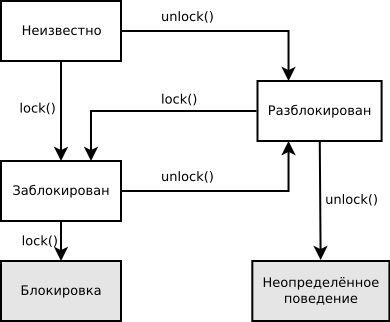
\includegraphics[width=0.6\linewidth]{lock-fsm}
   \caption{Конечный автомат проверки блокировки мьютекса}\label{pic:lock-fsm}
\end{figure}

Кроме того, данные проверок могут участвовать в определении достижимости состояний. Рассмотрим пример, затрагивающий опрос состояния потока ввода-вывода:

\begin{verbatim}
1   std::ifstream stream("/etc/apt/sources.list");
2   if (stream.is_open()) {
3     do_something();
4   }
5   if (stream.is_open()) {
6     stream.close();
7   }
\end{verbatim}

В результате моделирования файловых операций появляется предикат $isOpen(stream)$, значение которого связано с состоянием потока ввода-вывода \texttt{stream}. Однако, поскольку состояние объекта известно только проверке, выполняющей моделирование, условие достижимости ветвей зависит также от записи проверки в кортеже состояния программы.

В соответствии с новым определением состояния программы, введём новое определение эффекта. Эффект $e$ для состояния $S = \langle o, M, Expr, Rs, C \rangle$ определим следующим образом:

\begin{enumerate}
 \item $(\forall m \in M): m \rightarrow V$~--- эффект (запись символьного значения $V$ в область памяти $m$);
 \item $expr \rightarrow V$ в отношении $Expr$~--- эффект (появление нового активного выражения $expr$ со значением $V$ в $Expr$;
 \item $obj \rightarrow id$ в отношении $c_i$~--- эффект (изменение состояния объекта $obj$ в $id$ для проверки $c_i$);
 \item $e_1 \wedge \ldots \wedge e_n$~--- эффект, если $e_1, \ldots, e_n$~--- эффекты;
 \item $(Rs \wedge (\wedge_{i = 1}^n c_i)) \triangleright e$ является эффектом, если $Rs$~--- формула, $c_i$~--- предикаты $i$-й проверки, и $e$~--- эффект (эффект $e$ применим, если в текущем состоянии формула $Rs$ верна и состояние автоматов проверок допустимо).
\end{enumerate}

\subsection{Реализация формальной модели}

Clang Static Analyzer, являющийся основой для программной реализации разрабатываемых методов, также придерживается данной терминологии \cite{csa-base}. Каждому состоянию соответствует точка выполнения (\texttt{ProgramPoint}), для которого это состояние актуально. Точка выполнения может соответствовать выполняемому оператору (\texttt{PreStmt/PostStmt}), событию (например, вызову функции~--- \texttt{PreCall/PostCall}), изменению состояния проверки, и т.д. (Здесь и далее в скобках приводятся названия соответствующих классов из фреймворка Clang Static Analyzer). Переходы между состояниями обусловлены либо эффектами интерпретации отдельных выражений, определёнными стандартом языка, либо событиям, связанных с выполнением проверок проверяющими модулями (\texttt{Checker}). Из одной точки выполнения может идти не один переход в другое, а более~--- это происходит в случаях, когда условие перехода невозможно однозначно разрешить в пользу выбора какой-либо одной ветви выполнения, например, при обработке условных операторов (это и есть разделение на классы эквивалентности). Кроме того, проверки также могут разделять состояние программы, сохраняя в разных структурах состояния различающиеся данные состояния. Результирующее множество узлов в виде состояний и переходов из одного состояния программы в другое образует граф выполнения программы (\texttt{ExplodedGraph}).

За базовое моделирование процесса выполнения, без каких-либо проверок корректности исходного кода, отвечает ядро анализатора. Ядро анализатора представляет собой во-первых, набор методов, связанных с построением графа состояний выполнения программы (класс \texttt{CoreEngine}), а, во-вторых, набор методов, отвечающие за моделирование эффектов, специфичных для языка программирования, т.~е. моделирование эффектов выражений и правил их выполнения (класс \texttt{ExprEngine}). Кроме того, в процедуре построения графа выполнения могут принимать участие проверяющие модули, анализируя события, наступающие в процессе выполнения. Эти проверки могут останавливать построение графа на заданном пути в случае обнаружения критического дефекта, разделять состояние программы и вносить в него дополнительную информацию для работы проверяющего модуля.

Структура состояния является представлением состояния программы в точке выполнения. Структура состояния включает следующие данные:

\begin{enumerate}
 \item Содержимое памяти программы (модель памяти~--- \textit{RegionStore}) \cite{csa-store}, представляемое как отображение между регионами памяти и символьными значениями, связанными с этими регионами. Для создания записи в модели памяти необходимо произвести непосредственное связывание региона памяти и его значения, например, при обработке оператора присваивания. Операциями, изменяющими содержимое модели памяти, являются непосредственное связывание региона со значением (происходящее, например, при присваивании переменной значения), пометка регионов памяти как не содержащих первоначальное значение (инвалидация) и удаление имеющихся привязок, происходящее при потере регионом памяти активности, а также иногда используемое вместо инвалидации. В случае, если необходимо получить символьное значение для региона памяти, не имеющего записи в модели памяти (например, для аргументов функции), происходит неявное связывание с помощью символьного значения специального вида, при этом записи в модели памяти не создаётся.

 \item Окружение (\textit{Environment}) ставит в соответствие активным выражениям их символьные значения, как левосторонние, так и правосторонние: левосторонними значениями выражений являются абстрактные области памяти кода программы, где располагаются выражения, а правосторонними~--- вычисленные символьные значения выражений. Значения выражений, ставших неактивными, удаляются из окружения.
 
 \item Нетипизированное хранилище (\textit{GDM}, Generic Data Map) является контейнером для хранения данных проверок, а также используется для хранения некоторых специфических структур данных ядра анализатора, связанных с состоянием программы. Наиболее важными такими данными является карта соответствия символов и их множеств возможных значений, с помощью которой производится анализ достижимости. GDM позволяет хранить произвольные структуры данных, однако наиболее часто используются простейшие типы~--- указатели и целочисленные типы, а также неизменяемые словари, наборы и списки (\texttt{ImmutableMap}, \texttt{ImmutableSet} и \texttt{ImmutableList} соответственно), имеющие специальную поддержку, упрощающую их использование. За помещение данных в GDM и удаление их оттуда отвечают непосредственно использующие эти данные модули~--- проверки и модули ядра анализатора (в частности, ответственный за арифметические и логические вычисления решатель~--- \texttt{ConstraintManager}).
\end{enumerate}

Символьное значение является абстракцией переменного или константного значения какого-либо типа данных. Абстрактным значением можно представить, например, значение выражения, содержимое области памяти, саму область памяти и указатель на неё. В модели Clang Static Analyzer символьное значение может иметь несколько основные видов.

Первым видом символьных значений являются целочисленная константа. Используемый в работе символьный решатель Clang Static Analyzer на данный момент может корректно работать со значениями, представляемыми с помощью целочисленных и вещественных типов. Целочисленная константа имеет знаковость, разрядность и значение. Целочисленными константами также представляются символы строк (\texttt{char}-типы). Константы могут быть как правосторонними значениями (\texttt{nonloc::ConcreteInt}, \texttt{nonloc::ConcreteFloat}), так и левосторонними (\texttt{loc::ConcreteInt}~--- константные адреса памяти). Система арифметики позволяет производить вычисления над константами с использованием бинарных операторов с получением новой константы в качестве результата.

Собственно символьное значение (\texttt{SymbolVal}) является представлением для \textit{символьного выражения}, или \textit{символа}~--- абстрактного неконстантного выражения. Символьным выражением могут быть:

\begin{itemize}
 \item атомарный символ~--- атомарное правостороннее значение, которое нельзя однозначно определить как константу. Различные виды атомарных символов используются анализатором для различных целей. Существуют следующие виды атомарных символов:
 \begin{itemize}
 \item \texttt{SymbolRegionValue}~--- символ, являющийся значением некоторого региона памяти по умолчанию, если его исходное значение определено, но неизвестно, и не изменялось с момента начала анализа. Таким образом, в частности, представляются значения параметров функции на верхнем уровне стека вызовов;
 \item \texttt{SymbolExtent}~--- символ, представляющий размер соответствующего региона памяти в байтах, если этот регион имеет неконстантный (символьный) размер;
 \item \texttt{SymbolConjured}~--- символ, являющийся результатом выражения в случае, если правило вычисления данного выражения неивестно. В частности, \texttt{SymbolConjured} может быть получен в качестве возвращаемого результата функции, определение которой недоступно анализатору;
 \item \texttt{SymbolMetadata}~--- символ, описывающий некоторый регион памяти. Такие символы обычно используются проверяющими модулями для хранения информации об отслеживаемом регионе;
 \item \texttt{SymbolDerived}~--- символ, представляющий значение некоторого региона памяти, содержимое которого могло измениться с момента начала анализа неизвестным образом.
 \end{itemize}

 \item бинарное отношение символьного выражения и константы, выражаемое с помощью бинарных операторов (в CSA им соответствуют классы \texttt{SymIntExpr} и \texttt{IntSymExpr});
 \item бинарное отношение двух символьных выражений, представленную в виде бинарного выражения с помощью бинарных операторов (\texttt{SymSymExpr}).
\end{itemize}

Символьное выражение, таким образом, в общем случае представляет собой вычисляемое дерево, листьями которого являются атомарные символы и константы.

Ещё одним видом символьных значений являются значение вида региона памяти (\texttt{MemRegionVal})~--- значение, являющееся \textit{регионом памяти}, т.~е. абстрактным представления некоторого последовательного набора байт в памяти программы. Регион памяти является левосторонним выражением, будучи контейнером для некоторого значения, расположенного в памяти. Таким образом, регион памяти может быть как ключом для хранения в Store, так и его значением~--- например, значением указателя. В виде регионов памяти представляются левосторонние значения выражений (например, переменных, объектов). Каждый регион памяти, кроме \textit{областей памяти}, имеет родительский регион. Таким образом, регионы памяти образуют иерархию памяти, корневыми регионами которой являются области памяти, а прочие регионы памяти являются их подрегионами и подрегионами друг друга. Память делится на области согласно расположению объектов в оперативной памяти (таблица \ref{table:regionspace})

\renewcommand\arraystretch{1.2}

\begin{table} [htbp]
  \centering
  \parbox{15cm}{\caption{Виды областей памяти}\label{table:regionspace}}
%  \begin{center}
  \begin{tabular}{| l || p{0.6\linewidth} |}
  \hline
  \hline
  Название региона   & Хранимые данные \\
  \hline
  NonStaticGlobalSpaceRegion   & Глобальные переменные внешней области видимости  \\
  \hline
  StaticGlobalSpaceRegion      & Глобальные статические переменные    \\
  \hline
  HeapSpaceRegion  & Переменные, располагающиеся в <<куче>>    \\
  \hline
  StackArgumentsSpaceRegion & Переменные, являющиеся аргументами функции и располагающиеся на стеке   \\
  \hline
  StackLocalsSpaceRegion & Переменные, локальные для функции   \\
  \hline
  UnknownSpaceRegion & Вспомогательная область памяти для случаев, когда область хранения неизвестна \\
  \hline
  \hline
  \end{tabular}
%  \end{center}
\end{table}

Сами подрегионы разделяются на классы в зависимости от назначения (актуальные для C и C++ классы регионов перечислены в таблице \ref{table:memregions}. Вместе они образуют иерархию наследования. Классы регионов памяти играют важную роль при построении и применении резюме функций, поскольку несут в себе важную служебную информацию, необходимую для определения новых регионов в заданном контексте.

\begin{table} [htbp]
  \centering
  \parbox{15cm}{\caption{Виды регионов памяти}\label{table:memregions}}
%  \begin{center}
  \begin{tabular}{| l || p{0.6\linewidth} |}
  \hline
  \hline
  Название региона   & Хранимые данные \\
  \hline
  AllocaRegion   & Память на стеке, выделенная функцией \texttt{alloca()}  \\
  \hline
  SymbolicRegion      & Регион памяти, располагающийся по адресу, заданному указателем, который имеет символьное значение. Не имеет определённого размера и типа, они задаются его подрегионами    \\
  \hline
  BlockDataRegion  & Данные блоковых конструкций языка C и лямбда-выражений C++   \\
  \hline
  BlockTextRegion & Код блоковых конструкций языка C и лямбда-выражений C++   \\
  \hline
  FunctionTextRegion & Регион кода функции. Используется для операций взятия адреса функции   \\
  \hline
  CompoundLiteralRegion & Регион составного литерала \\
  \hline
  CXXBaseObjectRegion & Регион базового подобъекта класса. Задаётся определением базового класса \\
  \hline
  CXXTempObjectRegion & Регион временного объекта в C++ \\
  \hline
  CXXThisRegion & Регион, в котором располагается указатель \texttt{this} (C++). Используется при анализе методов класса вне контекста \\
  \hline
  FieldRegion & Регион поля структуры или класса. Задаётся определением поля \\
  \hline
  VarRegion & Регион переменной \\
  \hline
  ElementRegion & Регион элемента массива \\
  \hline
  StringRegion & Регион строкового литерала \\
  \hline
  \hline
  \end{tabular}
%  \end{center}
\end{table}


Для экономии ресурсов при обработке операций присваивания сложных объектов используются символьные значения отложенной обработки (\texttt{LazyCompoundVal}). Их задача заключается в отображении крупных блоков хранилища на другой регион памяти до момента, пока в новый регион памяти не будет произведена запись. Таким образом производится увеличение скорости работы анализатора за счёт уменьшения объёмов копируемой и хранимой в структуре состояния информации.

Вспомогательными видами символьных значений является неизвестное значение (\texttt{UnknownVal}) и неопределённое значение (\texttt{UndefinedVal}). Неизвестное значение является может являться результатом выражения, которое анализатор не может быть корректно смоделировано символьным решателем~--- например, битовые операции над неконстантными значениями; кроме того, неизвестное выражение может получиться, если операндом выражения является неизвестное выражение. Вместо неизвестного значения можно также создать новый атомарный символ без наложенных на него ограничений, что позволяет восстановить контекстную чувствительность для символьных операций. Неопределённое значение является результатом операций, результат которых не определён стандартом~--- в частности, разыменование нулевого указателя, получение значения неинициализированной переменной, а также при выполнении операций, операндом которого является другое неопределённое значение. Использование неопределённых значений также является одним из видов потенциальных проверок, и введение для этого отдельного типа символьного значения упрощает работу с анализатором.

Символьное значение можно получить следующими способами.

Левостороннее символьное значение можно получить при обращении к выражению, результат которого является левосторонним выражением (lvalue)~--- переменная, элемент массива, поле объекта и т.~д. При этом результирующее значение будет связано с объявлением той области памяти, к которой происходит обращение.

Символьное значение можно также получить в результате выполнения загрузки символьного значения из региона памяти (при преобразовании левостороннего выражения в правостороннее выражения, lvalue-to-rvalue cast). При этом, если регион уже имел непосредственную привязку, то будет получено символьное выражение, связанное с этой привязкой. В противном (и более частом) случае произойдёт создание атомарного символа, являющимся значением этого региона по умолчанию, без каких-либо наложенных на него ограничений, или возврат уже созданного символа.

Наконец, символьное значение можно получить, осуществив бинарную операцию над другими символьными значениями.

\subsection{Формальное описание процесса межпроцедурного анализа}

Пусть даны начальные состояния на момент вызова функции $s_{\text{вх}1}, \ldots, s_{\text{вх} n}$ и функция $F$ с последовательностью операторов $o_1, \ldots, o_m$. На основе этих входных данных дадим формальные определения рассматриваемых методов межпроцедурного анализа.

Межпроцедурный анализ с помощью метода встраивания подразумевает построение множества выходных состояний с помощью последовательного применения операторов функции к входным состояниям. Множество выходных состояний $S_{вых}$ для метода встраивания определяется следующим образом:

\begin{equation}
 S_{\text{вых}} = \lbrace S_{\text{вых}i} | \forall i \in [1, n]: S_{\text{вых}i} =  (o_m(o_{m-1}(\ldots (o_1(s_{\text{вх} i}))))) \rbrace.
\end{equation}


Межпроцедурный анализ с использованием резюме функции определим как применение композиции последовательности операторов функции к входным состояниям на момент вызова функции. Множество выходных состояний $S_{\text{вых}}$ для метода резюме определяется следующим образом:

\begin{equation}
S_{\text{вых}} = \lbrace S_{\text{вых}i} | \forall i \in [1, n]: S_{\text{вых}i} =  (o_1 \circ \ldots \circ o_m)(s_{\text{вх} i})) \rbrace.
\end{equation}

Важнейшее различие методов заключается в возможности метода резюме повторно использовать вычисленную композицию эффектов $(o_1 \circ ... \circ o_m)$ и применять её к различным состояниям.

\subsection{Эффекты, учитываемые в резюме функции}

Каждый оператор при своём выполнении производит эффект, заключающийся в изменении состояния программы. В случае анализа речь идёт о моделировании эффектов операторов, то есть о моделировании действия, которое моделируемый оператор оказывает на модель состояния программы.

С учётом описанной модели анализатора, сократить время анализа при использовании резюме в сравнении со встраиванием можно получить за счёт отсутствия необходимости затрачивать время на анализ эффектов, действия которых локальны или не учитываются при дальнейшем анализе. Например, связывание символьного значения с выражением имеет только локальный эффект, поскольку все выражения становятся неактивными при выходе из контекста анализа функции. Аналогично, локальный эффект имеют записи в локально видимую память и т.~д. Кроме того, модель анализатора заведомо допускает упрощения, поскольку анализатор не может досконально смоделировать поведение программы. Это означает, что ряд эффектов операторов не будет учтён, т.~е. на моделирование некоторых эффектов операторов будет затрачено время, однако результат этого моделирования не будет отражён в изменении состояния. Учёт этих упрощений и ограничений анализатора позволяет устранить непроизводительные затраты времени, поскольку при применении резюме непроизводительные вычисления не выполняются повторно. Возможно, однако, что некоторые эффекты самого применения резюме не могут быть учтены моделью анализатора и также будут отнесены к непроизводительным вычислениям. Тем не менее, время, затрачиваемое на применение резюме, по-прежнему не будет превышать время, требуемое на анализ вызова функции методом встраивания. Это объясняется тем, что набор эффектов, получаемых в результате применения резюме, включается строго или совпадает с набором эффектов, моделируемых при анализе методом встраивания.

В данной работе рассмотрен следующий набор эффектов, оказывающих влияние на состояние анализируемой программы в процессе её выполнения:

\begin{enumerate}
 \item Принятие решений о выборе пути выполнения. Выбор пути выполнения сопровождается наложением ограничений на символьные значения, относительно которых принимается решение о выборе пути. Если эти символьные значения содержат ссылки на внешние по отношению к вызываемой функции регионы памяти, накладываемые ограничения должны быть отражены в резюме. Кроме того, как было показано выше, каждое принятие решения влияет на присутствие и порядок операторов в последовательности выполнения, а следовательно, и на набор эффектов, включаемых в резюме. Наконец, наложение ограничений на входные данные функции в зависимости от выбора пути выполнения позволяет сохранить контекстную чувствительность при анализе, поскольку определённые пути выполнения могут быть достижимы лишь при ограниченном наборе входных значений аргументов функции и значений, находящихся во внешней по отношению к ней памяти.
 
 \item Модификация регионов памяти с областью видимости, отличной от локальной, то есть находящихся в статической или глобальной области видимости, принадлежащих куче, а также модификация аргументов, переданных по неконстантному указателю или неконстантной ссылке, и областей памяти, относящихся к ним (возможно, с использованием арифметики указателей).
 
 \item Инвалидация регионов памяти, то есть пометка некоторых регионов как изменивших значение на неизвестное. Данное действие обычно выполняется при моделировании оператора, все эффекты которого учесть по каким-либо причинам невозможно~--- например, при вызове функции с недоступным определением.
 
 \item Возврат вызываемой функцией некоторого значения. Это значение связывается с выражением вызова функции как элемент окружения.
 
 \item Пометки проверяющих модулей:
 
 \begin{enumerate}
  \item пометки символов, регионов памяти и символьных значений;
  \item события, которые необходимо проверить отложенно, когда контекст вызываемой функции станет достаточно определён для того, чтобы утверждать наличие потенциального дефекта;
  \item иные действия, связанные с процедурами проверок (в зависимости от логики работы проверяющего модуля).
 \end{enumerate}
 
\end{enumerate}

Поскольку проверяющие модули самостоятельно отвечают за свои данные, логику обработки резюме для проверок имеет смысл включать непосредственно в логику работы этих модулей.

Результирующий алгоритм применения резюме, учитывающий порядок применения различных эффектов, представлен на рис.~\ref{pic:summary-apply}


\begin{figure}
   \centering
   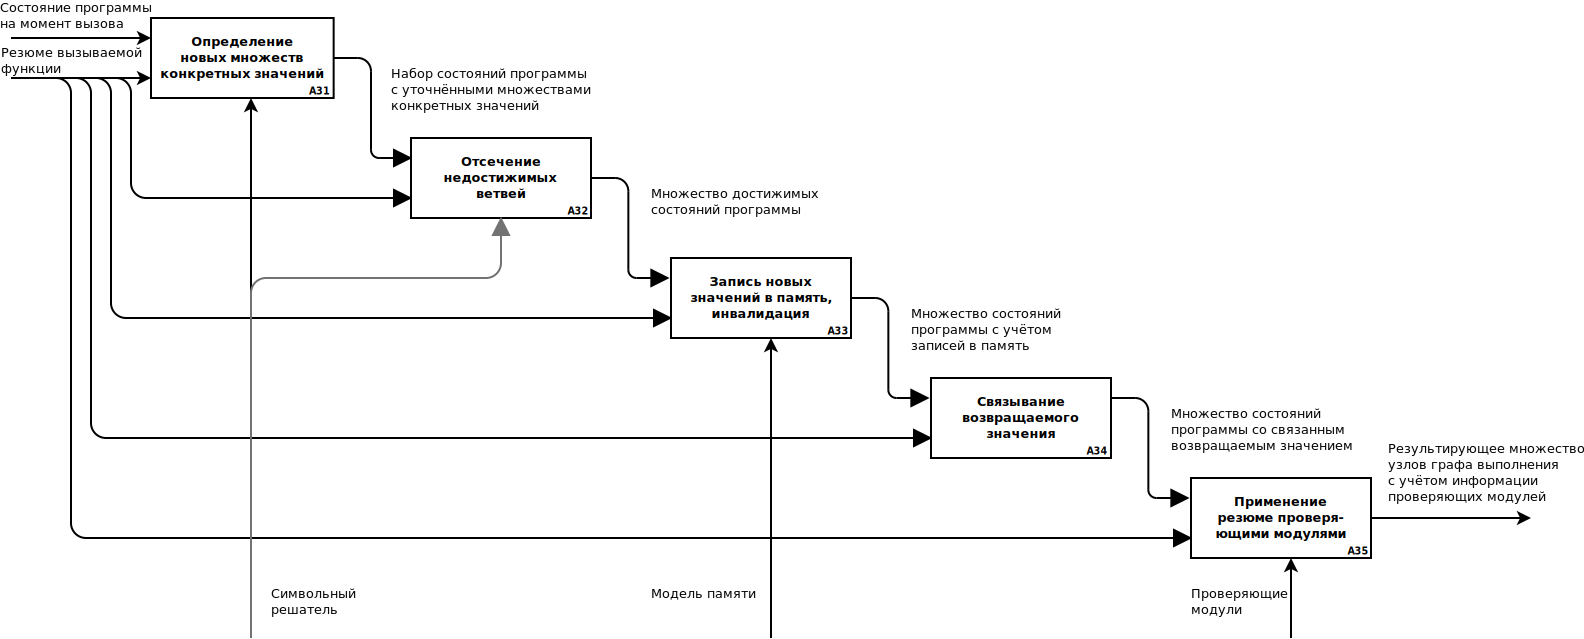
\includegraphics[width=\linewidth]{summary-apply.pdf}
   \caption{Последовательность применения резюме функции в разработанной модификации метода}\label{pic:summary-apply}
\end{figure}

\section{Оценка производительности методов межпроцедурного анализа}

На основании описания структуры данных состояния произведём оценку временной сложности алгоритмов анализа $T(N)$~--- функции времени выполнения от количества обрабатываемых узлов графа выполнения.  Для этого оценим два рассматриваемых методов межпроцедурного анализа~--- как использующего встраивание, так и использующего резюме вызываемой функции. $T(N)$ необходимо определить с точностью до коэффициентов линейной комбинации, а также оценить её поведение для различных случаев. Для этого рассмотрим основные структуры данных состояния~--- содержимое памяти, множество активных выражений и общее хранилище данных (GDM). С этими структурами данных в каждом из узлов графа выполнения могут быть произведены следующие операции:
\begin{enumerate}
 \item добавление во множество;
 \item удаление из множества;
 \item обращение к элементу множества.
\end{enumerate}

 Введём обозначения:

\begin {itemize}
 \item $N$~--- количество узлов графа выполнения;
 \item $S_i$~--- содержимое памяти в $i$-м узле графа выполнения;
 \item $|S_i|$~--- количество элементов (записей) в содержимом памяти $i$-го узла графа выполнения;
 \item $E_i$~--- множество активных выражений в $i$-м узле графа;
 \item $|E_i|$~--- количество элементов (записей) во множестве активных выражений в $i$-м узле графа;
 \item $C_{ik}$~--- множество элементов $k$-й проверки в $i$-м узле графа. В это множество входит также множество ограничений ($C_0$);
 \item $M$~--- количество проверок,
 \item $D$~--- глубина стека вызовов (вложенность вызова);
 \item $NParams_d$~--- количество аргументов $d$-й функции в стеке вызовов
\end {itemize}

Рассмотрим случай анализа одиночной функции вне контекста вызова. Поскольку все структуры данных представлены неизменяемыми словарями, временная сложность каждой из операций составляет $O(\log n)$, где $n$~--- количество элементов, хранящихся в словаре. При обработке каждого из узлов графа может быть произведено одно обращение, или одно добавление, или несколько удалений из содержимого памяти. Исключение составляет узел консервативного моделирования вызова функции, где может быть произведено несколько операций каждого вида. Кроме того, в каждом из узлов графа может произойти одно добавление записи во множество активных выражений, или несколько чтений из него, или несколько удалений. На основе этих данных суммарная асимптотическая сложность анализа графа выполнения функции ($\Theta(N)$) может быть оценена следующим образом:

\begin{equation}
 T(N) = \Theta \left(a_E \sum_{i=0}^N \log |E_i| + a_S \sum_{i=0}^N \log |S_i|  + a_C \sum_{i=0}^N \sum_{k=0}^M \log |C_{ik}|\right).
\end{equation}

В худшем случае элементы добавляются в множества в каждом узле графа выполнения и не удаляются оттуда до завершения анализа. Этот наиболее затратный случай, который мы примем за верхнюю оценку границы временной сложности ($O(N)$). В этом случае:

\begin{equation}
 T(N) = O \left(a_E \sum_{i=0}^N \log N + a_S \sum_{i=0}^N \log N  + a_C \sum_{i=0}^N \sum_{k=0}^M \log N \right),
\end{equation}

или, с точностью до коэффициентов, $T(N) = O(N \log N)$.

В лучшем случае, элементы будут добавляться и удаляться, сохраняя размер структур данных достаточно малым для константного времени операций. Этот случай мы примем за нижнюю границу временной сложности $\Omega$: $T(N) = \Omega(N)$.

Оценив сложность анализа графа выполнения заданного объёма, можно оценить сложность анализа вызова функции, имеющей заданный граф выполнения. Пусть функция анализируется относительно состояния $State'$ на момент вызова, которое имеет в модели памяти и в множестве активных выражений некоторые множества записей $S'$ и $E'$ соответственно. Аналогичные множества записей $C'_k$ будут существовать в структурах данных проверок.

\subsection{Оценка временной сложности реализации алгоритма метода встраивания}

При использовании встраивания функции для каждого вызова функции в модели памяти дополнительно создаётся отображение фактического аргумента на формальный параметр функции, и количество таких отображений равно количеству параметров функции. Поэтому асимптотическая временная сложность анализа графа выполнения будет следующей:

\begin{equation}
\label{eq:inlining-full}
\begin{split}
 T(N) = \Theta \left( a_E \sum_{i=0}^N \log \left(\sum_{d = 0}^D |E'_d| + |E_i| \right) + \right. \\
 + a_S \sum_{i=0}^N \log \left(\sum_{d = 0}^D \left(|S'_d| + NParams_d \right) + |S_i|\right)+ \\
 + \left.a_C \sum_{i=0}^N \sum_{k=0}^M  \log \left(\sum_{d = 0}^D |C'_d|  + |C_{ik}|  \right) \right),
 \end{split}
\end{equation}

Из полученного соотношения следует, что рост отдельных компонентов временной составляющей является логарифмическим. Однако стоит отметить два фактора, негативно влияющих на производительность в случае встраивания.

\begin{enumerate}
 \item Зависимость производительности анализа от вложенности вызова.
 \item Глубина вложенности вызовов и объёмы структур данных редко бывают большими (чаще они содержат до 10 элементов). На этом диапазоне зависимость от размера для логарифмической функции более значительна, чем при больших объёмах данных.
\end{enumerate}


\subsection{Оценка асимптотической сложности реализации алгоритма разрабатываемого метода, использующего резюме}

Оценим аналогичным образом временные затраты на применение резюме функции и его сбор.

В резюме может вноситься подмножество записей из модели памяти, относящееся к нелокальным для функции адресам ($\widehat{S} \in S$), а также некоторое подмножество записей из данных проверок $\widehat{C}_k \in C_k$. В худшем случае, $\widehat{S} \equiv S$ и $\forall k: \widehat{C}_k \equiv C_k$, и все узлы графа выполнения являются конечными. Несмотря на невозможность данной ситуации, она позволяет произвести оценку асимптотической сложности сверху:

\begin{equation}
 T(N) = O \left(a_S \sum_{i=0}^N \log N  + a_C \sum_{i=0}^N \sum_{k=0}^M \log |C_{ik}| \right).
\end{equation}

Однако, стоит отметить, что вместо непосредственного сбора резюме проверяющими модулями может использоваться информация о состоянии непосредственно в конечных точках. В этом случае сложность сбора резюме уменьшается до:

\begin{equation}
 T(N) = O \left(a_S \sum_{i=0}^N \log N  + a_C \sum_{i=0}^N  \log |C_{0k}| \right).
\end{equation}

Оценим теперь сложность применения резюме вызываемой к состоянию на момент вызова. Применение резюме в этом случае сводится к обновлению структуры состояния $S'$ и данных проверок $C'_{ik}$:

\begin{equation}
\label{eq:summary-apply}
\begin{split}
 T(N) = O \left( a_S \sum_{i=0}^N \log \left(|S'| + |S_i|\right) +  a_C \sum_{i=0}^N \sum_{k=0}^M  \log \left(|C'|  + |C_{ik}|  \right) \right).
 \end{split}
\end{equation}

Несмотря на схожесть формул \ref{eq:summary-apply} и \ref{eq:inlining-full}, формула \ref{eq:summary-apply} представляет собой оценку сверху. Хотя логарифмический вид асимптоты сохраняется, на основе сравнения этих формул можно выделить ряд преимуществ метода резюме:

\begin{enumerate}
 \item Зависимость производительности анализа от вложенности вызова при использовании резюме отсутствует.
 \item Использование резюме исключает обработку операторов и работу с множеством активных выражений. По данным замеров производительности, эта часть работы анализатора занимает более 30\% времени.
\end{enumerate}

Данные расчёты позволяют выявить основные источники прироста производительности при использовании резюме даже в худшем случае. Кроме того, необходимо учесть, что худший для резюме случай встречается крайне редко. Обычно, множества $\widehat{S}$ и $\widehat{C}$ представляют собой достаточно небольшую часть множеств $S$ и $C$ соответственно. Поскольку теоретическую оценку среднего случая дать крайне затруднительно, более подробно производительность методов в среднем случае оценена при анализе большой репрезентативной кодовой базы (ОС Android) в главе 4.

\section{Порождение новых ветвей выполнения программы и отсечение недостижимых путей}

Одним из результатов сбора резюме являются пары <<регион памяти~--- символьное значение>>. В результате актуализации символьных значений из резюме могут получиться символьные значения, имеющие множества конкретных значений, отличные от множеств конкретных значений этого символьного значения в контексте вызывающей функции. Это является следствием того, что при моделировании условий внутри вызываемой функции может произойти разделение входных данных функции (аргументов и внешних переменных) на классы эквивалентности.

Рассмотрим пример. Пусть вызывается функция:

\begin{verbatim}
     1  void f(int a) {
     2    if (a > 10) {
     3      …
     4    } else {
     5      …
     6    }
     7  }
\end{verbatim}

В результате анализа этой функции в её резюме войдут две ветви выполнения. В первой ветви \texttt{a} будет иметь диапазон конкретных значений от \texttt{INT\_MIN} до 10, во второй~--- от 11 до \texttt{INT\_MAX}.

Пусть происходит вызов функции при \texttt{a} от 5 до 13. Тогда в первой создаваемой ветви выполнения \texttt{а} будет иметь диапазон от 5 до 10, а во второй~--- от 11 до 13.

Далее, пусть в вызывающей функции \texttt{a} имеет диапазон конкретных значений от 5 до 9. Тогда в первой ветви выполнения \texttt{a} будет иметь диапазон от 5 до 9, а во второй ветви выполнения множество значений будет пустым. Наличие символьного значения с пустым множеством допустимых значений означает, что вторая ветвь является недостижимой и может не рассматриваться. Действительно, при вызове функции при заданном \texttt{а} выполняется только \texttt{else}-ветвь, но не \texttt{if}-ветвь.

% Рассмотреть отдельную ветвь и убрать i.
Введём следующие обозначения:
\begin{itemize}
 \item $n$ – количество ветвей выполнения, полученных в резюме анализа вызываемой функции,
 \item $i$ – номер ветви выполнения, где $0 \leqslant i < n$,
 \item $p_i$ – количество символьных правосторонних входных значений в $i$-ой ветви выполнения,
 \item $j$ – номер символьного значения, где $0 \leqslant j < p_i$,
 \item $s_{ij}$ – символьное значение с номером $j$ в $i$-ой ветви выполнения,
 \item $r_{\text{входные}\ ij}$ – множество значений для $s_{ij}$ в контексте вызывающей функции в точке непосредственно перед вызовом функции,
 \item $r_{\text{резюме}\ ij}$ – множество значений для $s_{ij}$ в контексте вызываемой функции,
 \item $state_{\text{входное}}$~--- состояние программы в контексте вызывающей функции в точке непосредственно перед вызовом функции,
 \item $state_{\text{выходное}}$~--- состояние программы после вызова функции (после применения резюме).

\end{itemize}

Тогда при применении $i$-й ветви выполнения резюме:

\begin{equation*}
\label{result_sval}
 \forall i \in [0; n], \forall j \in [0; p_i]:\ r_{\text{выходные}\ ij} =  r_{\text{входные}\ ij} \cap r_{\text{резюме}\ ij},
\end{equation*}

то есть результирующее множество является пересечением множеств входных конкретных значений символического значения и множества конкретных значений символического значения из применяемой ветви резюме.

В случае, если результирующее множество конкретных значений является пустым хотя бы для одного символического значения, то данная ветвь выполнения является недостижимой и не принимается в дальнейшее рассмотрение, что может быть выражено формулой \ref{empty_set}.

\begin{equation*}
 \label{empty_set}
 (\exists i, j: r_{\text{входные}\ ij} \cap r_{\text{резюме}\ ij} = \varnothing)  \Rightarrow (state_{\text{входное}} \nrightarrow state_{\text{выходное}})
\end{equation*}


\section{Сбор данных для создания резюме}

Пусть некоторое значение относится к региону памяти. Поскольку при передаче аргумента в функцию не по значению его значение может измениться, необходимо различать входное значение региона до его изменения в функции и выходное значение. Для получения информации о разбиении данных на классы эквивалентности можно отслеживать события ветвлений (assume), однако данный подход неудобен на практике, поскольку, во-первых, требует отдельного отслеживания событий изменений региона для разделения входных и выходных значений, и, во-вторых, требует активного участия сборщика резюме в процессе принятия решения о ветвлении. Вместо этого в настоящем решении предложен и использован подход, основанный на проверке активности символов и регионов. Поскольку входные данные, внешние по отношению к анализируемой функции, всегда являются символическими, отслеживая событие потери актуальности (активности), можно определить множество возможных конкретных значений символа, связанного с данным регионом, в данной ветви выполнения. При этом первое событие потери активности соответствует множеству входных значений, а последнее соответствует множеству выходных значений, причём если они совпадают, это означает, что никаких присваиваний или инвалидаций региона входного символа не было, и входное множество является также выходным множеством. Данный метод позволяет избежать использования сложных алгоритмических схем для сбора входных и выходных значений аргументов функций, а также входных значений глобальных регионов памяти.

Сбор выходных значений также бывает необходимо проводить по окончании пути выполнения функции. Это необходимо для обработки символьных значений, привязанных к региону памяти непосредственным присваиванием или иным видом связывания. Для этого используется итерация по хранилищу с сохранением множеств конкретных значений внешних по отношению к функции регионов памяти в резюме. 

Инвалидация региона памяти в терминологии Clang Static Analyzer означает связывание с данным регионом нового символа, без наложенных на него ограничений, т.~е. способного принимать произвольные значения. Поскольку символьные значения, связанные с регионами памяти, обрабатываются при завершающем проходе по хранилищу, а значения регионов, актуальные до инвалидации, обрабатываются по событию потери активности, непосредственно предшествующему событию связывания нового значения, инвалидация обрабатывается автоматически, и дополнительных действий для обработки инвалидаций регионов памяти не требуется.

Обработка события возврата функцией значения достаточно тривиальна. Результирующее символьное значение сохраняется в резюме целиком, а ограничения, накладываемые на него и на его части, обрабатываются отдельно.

За хранение данных проверок проверяющие модули отвечают самостоятельно. Основными видами данных проверок является отметка отложенной проверки и данные состояния проверки. Отложенные проверки используются для выдачи предупреждений в тех ситуациях, когда из-за отсутствия данных о контексте вызова невозможно однозначно утверждать наличие дефекта или его отсутствие. Данные, находящиеся в состоянии программы на момент окончания анализа пути выполнения, используются для построения нового состояния проверки при применении резюме. 

\section{Актуализация символьных значений}

В результате сбора резюме на предыдущем шаге мы получаем некоторое множество регионов памяти, с которыми связаны некоторые символьные значения. Кроме того, регионы памяти сами могут входить в символьные значения как их составная часть. Однако, полученные регионы памяти адресуются в контексте объявлений имён внутри функции. В контексте вызывающей функции эти регионы могут иметь уже другое значение, то есть регионы, используемые внутри функции, являются относительными по отношению к вызывающей функции. Так, например, в контексте вызываемого метода класса регион памяти, связанный с указателем \texttt{this}, будет адресоваться безотносительно какого-либо объекта, а в контексте вызывающей функции этот регион будет регионом, в котором находится объект, метод которого вызывается. Аналогично, аргумент функции, фигурирующий в ней как самостоятельная переменная, (и, соответственно, как самостоятельный регион памяти), может быть подрегионом в контексте вызывающей функции~--- полем структуры, элементом массива. Кроме того, с регионом памяти в контексте вызываемой функции может быть связан не символ, относящийся к региону памяти, а константа, символьное выражение или иное значение, не имеющее в своей основе регион аргумента. Всё это означает, что для корректного применения резюме необходимо производить актуализацию символьных значений, то есть их перевод из контекста имён и значений вызываемой функции в контекст имён и значений вызывающей функции.

Идея актуализации заключается в следующем. Пусть имеется символьное значение. В его состав могут входить символы, регионы памяти и константы. Они, согласно модели анализатора, образуют дерево. Непосредственно актуализации подвергаются только регионы памяти. Таким образом, в символьном значении происходит подмена регионов памяти, содержащихся в нём, на актуализированные. Затем, если это возможно, символы полученного символьного выражения вычисляются в константы, заменяя исходные поддеревья. Данную процедуру можно выразить следующим алгоритмом:

\begin{enumerate}
 \item Для всех регионов памяти, содержащихся в символьном значении:
 \begin{enumerate}
  \item Создать новый регион, являющийся актуализацией данного региона.
  \item Заменить в символьном значении исходный регион актуализированным.
 \end{enumerate}
 \item Для всех символов, содержащихся в символьном значении, полученном на шаге 1:
  \begin{enumerate}
  \item Проверить, не вычисляется ли символ в константу.
  \item Если символ вычисляется в константу, заменить данный символ вычисленной константой.
 \end{enumerate}

\end{enumerate}

В соответствии с типами символьных значений, можно производить актуализацию символьных значений в зависимости от их типа.

Константные значения являются неизменяемыми при их актуализации, поскольку они не содержат элементов, зависящих от контекста. Вместе с тем, типы константного значения в контексте вызываемой функции и в контексте вызывающей функции могут быть различающимися, поэтому может понадобиться осуществление дополнительного приведения типов для константы.

Символьные значения, относящиеся к регионам памяти, можно актуализировать, используя следующие правила для различных категорий регионов памяти.

\subsection{Регионы, относящиеся к пространству аргументов вызываемой функции}
 
Можно выделить два различных случая передачи, в зависимости от того, является ли передаваемый тип ссылочным или типом указателя, или не является.
 
В случае, если аргумент передаётся по ссылке, левостороннее значение фактического аргумента становится левосторонним значением формального параметра, а правостороннее значение фактического параметра становится правосторонним значением формального параметра. Это значит, что значение объекта в результате выполнения функции может отличаться от значения на момент вызова, поскольку в результате передачи по ссылке с фактическим аргументом может быть связано другое значение.

Таким образом, при передаче аргумента по ссылке:
\begin{enumerate}
 \item Адрес формального параметра является адресом фактического аргумента.
 \item Левостороннее значение формального параметра является левосторонним значением фактического аргумента.
 \item Правостороннее значение формального параметра является правосторонним значением фактического аргумента.
 \item Базовым регионом для построения подрегионов доступа, относящихся к региону памяти формального параметра, является левостороннее значение фактического аргумента.
\end{enumerate}

В случае, если аргумент передаётся по указателю, правостороннее значение фактического параметра становится правосторонним значением формального параметра. Для левосторонних значений данное утверждение неверно: выполнение присваивания формальному аргументу внутри функции не влияет на значение фактического аргумента. Однако в случае, если указываемый тип не является константным, в результате вызова функции может измениться привязка региона памяти, адрес которой задаёт указатель, и его субрегионов.

Таким образом, при передаче аргумента по указателю:
\begin{enumerate}
 \item Правостороннее значение формального параметра является правосторонним значением фактического аргумента.
 \item Регион памяти с адресом, задаваемым указателем формального аргумента является регионом памяти с адресом, задаваемым указателем фактического аргумента (поскольку значения указателей совпадают). Привязки этого региона и его субрегионов могут изменяться в зависимости от модификатора константности их типов.
 \item Базовым регионом для построения подрегионов доступа, относящихся к региону памяти с адресом, задаваемым указателем формальным параметром, является регион памяти с адресом, задаваемым указателем фактического аргумента.
\end{enumerate}

В случае, если аргумент передаётся по значению правостороннее значение фактического параметра становится правосторонним значением формального параметра.

В случае передачи в качестве аргумента структурных типов по ссылке или указателю, правила изменения их полей аналогичны. Так, в случае передачи по значению структуры, содержащей ссылку в качестве поля, данное поле можно считать передающимся по ссылке. Фактически, в случае структурных типов можно считать, что передаётся набор аргументов по их типам с тем отличием, что при потере актуальности их окружающего региона памяти эти поля также могут потерять актуальность.

\subsection{Регионы памяти внешней области видимости}

Помимо передаваемых аргументов, вызываемая функция может иметь доступ к ряду других данных~--- переменных, имеющих области видимости выше, чем функция. К этим регионам относятся глобальные переменные и члены класса и его предков, если вызываемой функцией является метод класса. Их изменения и наложения ограничений на них также необходимо отслеживать.

Регионы глобальных переменных (включая статические) сохраняются неизменными, дополнительные действия по из актуализации предпринимать не нужно. Это так, поскольку регионы глобальных переменные не зависят от контекста вызова и связаны лишь с объявлением соответствующих переменных.

Методам класса, включая конструкторы, деструкторы и операторы-члены класса, могут быть доступны для чтения и записи поля как самого класса, так и его предков в иерархии наследования. При актуализации регионы памяти, относящиеся к статическим полям класса, не изменяются, поскольку они не относятся к конкретному объекту поля и, следовательно, их адресация не зависит от контекста вызова. Нестатические поля в контексте вызываемого метода адресуются относительно условного объекта, связанного с указателем \texttt{this}, и, поскольку в контексте вызываемой функции фактическим объектом будет объект, метод которого вызывается, при актуализации эти поля становятся соответствующими полями вызываемого объекта. Если определение нестатического поля принадлежит классу, определение которого находится ниже по иерархии наследования, то поле отображается в соответствующее поле родительского класса объекта в соответствии с компоновкой полей дочернего класса.

\subsection{Актуализация составных и служебных символьных значений}

Актуализация символьных значений, обозначающих бинарные операции над символами (бинарные символьные значения), выполняется следующим образом. Сначала выполняется актуализация правой и левой частей символьного значения. Если результатом бинарной операции является константа, эта константа становится результирующим символьным значением. В противном случае результатом актуализации является новое символьное значение в виде бинарной операции. Фактически, бинарные символы актуализируются рекурсивно, с возможными упрощениями в виде свёртывания отдельных элементов или всего выражения в константу. Это свёртывание объясняется уменьшением множеств входных значений каждого из символьных значений, входящего в состав бинарного символьного значения, при уточнении контекста вызова.

Актуализация метасимволов является отдельной подзадачей. Под метасимволами понимают символические значения, относящиеся к объекту анализа, но не являющиеся его непосредственной характеристикой. Выделение метасимволов связано с тем, что источником метаданных является не ядро анализатора, а сами проверяющие модули, которые связывают необходимую информацию в виде метасимволов с интересующими их регионами памяти и выражениями. Соответственно, регионы памяти и выражения могут иметь более одного связанного с ними метасимвола. Поскольку каждый проверяющий модуль может реализовывать свой подход к использованию метаинформации и обозначениям интересующих его объектов, для актуализации метасимволов используется отдельное событие, на которое должны подписываться проверяющие модули, использующие метаданные. В результате проверяющие модули самостоятельно обновляют представление связанных с ними символьных значений и нарушение принципа инкапсуляции данных не происходит. В качестве примера можно привести проверку, связанную с длиной строки. Длина строки не входит в число данных, о которых известно самому анализатору~--- за её моделирование отвечает проверяющий модуль, связывающий символьное значение (метасимвол) с регионом памяти данной подстроки. Таким образом, задачей проверяющего модуля при актуализации метазначения, связанного с регионом, является поиск существующего метазначения для этого региона и его возврат.

Построение и актуализация сложных структур данных в резюме производится с помощью сохранения цепочки родительских регионов. Для каждого региона памяти, имеющего связанное с ним символьное значение (как явно, так и неявно), строится упорядоченный список родительских регионов, начиная от региона верхнего уровня~--- $M_0 \ldots M_n$. При этом регионы $M_1 \ldots M_n$  может быть только регионами элемента массива, регионами поля структуры или регионами данных базового класса. Этот список сохраняется в резюме и используется для актуализации значений по следующему алгоритму.

\begin{enumerate}
 \item Актуализация региона $M_0$.
 \item Для всех регионов $M_1 \ldots M_n$ согласно их положению в списке:
 \begin{enumerate}
  \item если $M_i$~--- регион элемента массива, то в резюме сохраняется символьное значение индекса, а результатом актуализации является элемент массива от региона, полученного на $(i-1)$-ом шаге алгоритма, с символьным значением индекса, полученным в результате актуализации сохранённого значения индекса.
  \item если $M_i$~--- регион поля структуры, то в резюме сохраняется объявление поля структуры, а результатом актуализации является поле структуры от региона, полученного на $(i-1)$-ом шаге алгоритма, с тем же определением.
  \item если $M_i$~--- регион данных базового класса, то в резюме сохраняется ссылка на определение базового класса, а результатом актуализации является подрегион данных базового класса от региона, полученного на $(i-1)$-ом шаге, с тем же определением.
 \end{enumerate}
\end{enumerate}

Цепочка родительских регионов может строиться как явно~--- при построении резюме для региона памяти, так и неявно~--- при сохранении и последующем разборе символьного значения, для которого строится резюме.

\subsection{Актуализация литеральных регионов}

Литеральные регионы, т.~е. регионы, относящиеся к строковым или составным литералам, актуализируются с использованием выражения языка, по которому они были построены. Поскольку эти регионы хранят исходное выражение как служебную информацию, именно это выражение записывается в резюме, и по нему строится актуализированное выражение. Фактически, литералы не изменяются вместе с контекстом, и обычно хранятся в статической памяти, являясь видом констант, что упрощает работу с ними при использовании метода резюме.

\section{Применение резюме проверяющими модулями}

Схемы применения резюме, описанные выше, затрагивают отсечение недостижимых ветвей выполнения программы и уточнение множества конкретных значений для символьных значений. Однако для того, чтобы анализатор имел возможность выполнять проверки при вложенном вызове функции, необходима доработка проверяющих модулей. Для получения проверяющими модулями возможностей анализа при использовании резюме мы вводим две дополнительных функции обратного вызова. Первая из них (названная \texttt{evalSummaryPopulate}) вызывается для сбора резюме проверяющим модулем, вторая (названная \texttt{evalSummaryApply}) вызывается при применении резюме.

Проверяющий модуль, имеющий возможность выполнения действий при событии \texttt{SummaryPopulate}, должен сохранить информацию, которая может понадобиться для обновления состояния или для выполнения отложенной проверки. Информация, содержащая в резюме, не освобождается до окончания работы анализатора, поэтому проверяющий модуль может использовать произвольный формат хранения данных, лучшим образом отвечающий задаче проверки. Как показала практика модификации проверяющих модулей, для каждой проверки, проводимой модулем, в GDM обычно помещается две дополнительных записи, которые затем будут использоваться для заполнения резюме~--- для обновления состояния и для отложенной проверки. В качестве примера рассмотрим проверку двойного закрытия файлового дескриптора. В резюме помещаются две секции: первая отвечает за обновление состояния дескриптора (является ли он открытым или закрытым), а вторая~--- за выполнение отложенной проверки: в ней запоминаются события закрытия дескрипторов, исходное состояние которых неизвестно.

При обработке события \texttt{SummaryApply} проверяющий модуль должен произвести обновление состояния в соответствии с информацией, хранящейся в выбранной ветви резюме. Так, если при выполнении вызова функции дескриптор был закрыт, он должен быть помечен как закрытый в состоянии вызывающей функции. Если же в контексте вызывающей функции уже известно, что дескриптор закрыт, то отложенная проверка должна выдать предупреждение.

Кроме того, если проверяющий модуль использует метаданные для хранения информации о состоянии контролируемых объектов, он может потребовать реализации функциональности актуализации метасимвола. Для этого вводится функция обратного вызова \texttt{evalSummarySVal}. Реализующие эту функциональность модули должны определять, на какое символьное значение метаданных отображается актуализированный метасимвол, и возвращать это символьное значение в качестве результата функции обратного вызова. Пример использования данной функции приведён в описании реализации проверки переполнения строки C++ (раздел \ref{sect:basic_string}).

Интерес представляет сравнение двух методов обработки данных проверяющими модулями. Определим два вида проверок формально.

Проверку при использовании метода встраивания определим следующим образом. Пусть имеется граф выполнения программы в виде дерева. Алгоритм поиска осуществляет обход дерева от корня к листу по пути $w$ без возврата, собирая ограничения, наложенные на входные данные, и отслеживая изменение состояния программы в каждом узле графа выполнения. Алгоритм поиска выдаёт срабатывание в случае обнаружения нарушения заданного для него условия корректности состояния программы в заданной точке, таким образом представляя дефект конъюнкцией $pre_w \wedge node_w$, т.~е. отображением множества значений входных данных функции на узел графа выполнения, состояние которого нарушает условие корректности программы.

Проверку при использовании метода резюме определим как проверку при использовании метода встраивания для функции верхнего уровня и отложенную проверку при использовании межпроцедурного вызова. Под отложенной проверкой понимается дополнительная проверка всех узлов графа выполнения вызываемой функции в узле применения резюме с актуализацией состояния в данных узлах с учётом контекста вызова и актуализированных ограничений на момент выхода из вызываемой функции. Отложенная проверка и обычная проверка производятся с использованием одного критерия корректности состояния программы.

\textbf{Утверждение 1}. Если при использовании проверки с помощью метода встраивания результатом проверки является предупреждение, выданное в некотором узле графа выполнения программы, то при использовании метода резюме для той же функции верхнего уровня и того же набора вызываемых функций результатом проверки методом резюме также является предупреждение, выданное в узле графа выполнения вызывающей функции или в одном из узлов графов выполнения вызываемых функций.

\textbf{Доказательство}. В результате применения резюме в идеальном случае (т.~е., при отсутствии ограничений на количество анализируемых узлов графа) состояние в каждом из создаваемых узлов применения резюме будет аналогичным состоянию одного из узлов выхода из функции графа выполнения программы при использовании метода встраивания. Из данного утверждения следует, что обычная проверка функции верхнего уровня и проверка при использовании метода встраивания будут иметь одинаковый результат для всех общих узлов графа выполнения функции верхнего уровня, если дефект находится в одном из таких узлов. Докажем теперь, что отложенная проверка выдаёт срабатывания для остальных случаев срабатывания проверки метода встраивания. Пусть состоянию программы на момент вызова функции $St_{caller}$ соответствует набор ограничений множества входных данных $pre_w$, а узел срабатывания $node_{w'}$ достижим на пути $w'$ вызываемой функции при ограничениях множества входных данных функции $pre_{w'}$. Тогда узел срабатывания графа при вызове функции достижим при входных данных 
\begin{equation}
 \label{form:pre-inlining}
 pre_{node} = pre_w \wedge pre_{w'}
\end{equation}
Данные ограничения выполняются непосредственно для метода встраивания. В случае использования метода резюме узлу вызываемой функции могут соответствовать $n$ ветвей выполнения, где $n \geqslant 1$. Поскольку эти ветви имеют общего предка, ограничения множества входных данных этих ветвей графа выполнения функции образуют набор ограничений, для которого выполняется условие 
\begin{equation}
 pre_{w'} = \bigvee_{i = 1}^n pre_{w'_i},
\end{equation}

откуда

\begin{equation}
\label{form:inclusion}
 \forall i \in [1, n]: pre_{w'_i} \subseteq pre_{w'}
\end{equation}

Поскольку отложенная проверка проводится с ограничениями произвольно выбранной ветви графа выполнения $pre_{w'_i}$, актуализированные ограничения будут соответствовать предусловиям 
\begin{equation}
 pre_{w_i} = pre_w \wedge pre_{w'_i},
\end{equation}

откуда, с учётом \ref{form:pre-inlining} и \ref{form:inclusion}, получаем

\begin{equation}
\label{form:total-inclusion}
 pre_{w_i} \subseteq pre_{node}.
\end{equation}

Неравенство \ref{form:total-inclusion} означает, что ограничения при отложенной проверке входят в ограничения при обычной проверке метода встраивания, и входят в класс эквивалентности данных ограничений. Если нарушение правила корректности обнаружено при входных ограничениях $pre_{node}$, оно будет обнаружено при любых входных данных заданного класса эквивалентности. Следовательно, если нарушение правила происходит при использовании метода встраивания, оно будет обнаружено и при использовании метода резюме. Утверждение доказано.

Обратное утверждение, вообще говоря, не является верным. Рассмотрим пример.

\begin{verbatim}
  1  int callee(int *p) {
  2    int t = *p;
  3    if (p)
  4      return t;
  5    return 0;
  6  }
  7
  8  int caller(int *p) {
  9    return callee(p);
 10  }
\end{verbatim}

Пусть задачей проверяющего модуля является проверка на разыменование нулевого указателя. В случае использования МПА методом встраивания дефект обнаружен не будет, поскольку на момент разыменования \texttt{p} неизвестно, является ли он нулевым или нет. Однако при использовании МПА методом резюме в резюме функции будет записаны две ветви: $(p = 0 \wedge 0) \vee (p \neq 0 \wedge *p)$. Поскольку на момент разыменования неизвестно, является ли указатель нулевым или нет, для обеих ветвей резюме планируется отложенная проверка. При применении первой ветви резюме значение указателя актуализируется в 0, поскольку ограничений в вызывающей функции на него не имелось, и отложенная проверка даст срабатывание на разыменование нулевого указателя. Причина подобного различия в поведении заключается в том, что при использовании МПА методом резюме на момент вызова функции имеется больше информации об ограничениях множества входных данных, которые используются в вызываемой функции.

\textbf{Утверждение 2}. При использовании отложенной проверки в конце анализа функции верхнего уровня при использовании МПА методом встраивания и МПА методом резюме множества срабатываний совпадают.

\textbf{Доказательство}. Поскольку в идеальном случае актуализация состояния при использовании резюме даёт набор состояний, соответствующих состояниям программы после межпроцедурного анализа методом встраивания, в конце анализа функции верхнего уровня множества классов эквивалентности разбиения входных данных функции и листьев графа выполнения должны совпадать. В конце выполнения функции ряд классов эквивалентности, соответствующий листьям-наследникам узла отложенной проверки, будет входить в класс эквивалентности, при котором был обнаружен дефект при использовании метода резюме. Следовательно, при повторной проверке будет установлено наличие дефекта.

\section{Методы реализации резюме для различных видов проверок}

Как говорилось выше, проверяющие модули должны самостоятельно обеспечивать поддержку резюме. В настоящем разделе дано описание разработанных в рамках данной работы и апробированных методов обеспечения резюме в проверяющих модулях различного назначения. Данные проверяющие модули были ранее разработаны в Московском исследовательском центре Samsung в рамках исследовательских работ и адаптированы к МПА методом резюме в рамках данной работы. На примере этих проверяющих модули продемонстрируем ряд разработанных общих техник для эффективного использования резюме в проверяющих модулях при использовании межпроцедурного анализа. Комбинируя данные техники, можно эффективно реализовывать метод резюме для проверок различного назначения, от проверок ошибок при работе с памятью до проверки корректности работы с механизмом исключений и поиска ошибок, связанных с многопоточностью.

\subsection{ConstModifiedChecker~--- проверка модификации константных данных}

Задачей данной проверки является определение записи в область памяти, имеющую константный квалификатор, с использованием приведения типа к неконстантному (CERT EXP05-C согласно классификации CERT \cite{cert}). Данная проверка преследует две цели. Во-первых, модификация данных таким образом представляет собой плохой стиль програмирования и указывает на необходимость пересмотра интерфейсов программы; в случае константного метода класса (C++) в ряде случаев нужный эффект можно получить, используя ключевое слово \texttt{mutable} для определения члена класса, который может быть изменён при вызове семантически константного метода. Во-вторых, попытка записи в память, инициализируемую компилятором как константную, с использованием приведения типов, приводит к неопределённому поведению и к ошибке сегментации, поскольку объект может быть помещён в память только для чтения \cite{c-std}.

Исходный принцип действия проверки следующий. Проверка отслеживает все регионы памяти, встречаемые в процессе анализа программы и имеющие изначально константный тип. Данные регионы записываются в GDM. В случае выполнения явного приведения типов (с использованием одного из выражений \texttt{ExplicitCastExpr})~--- с использованием приведения типов в стиле C, операторов \texttt{const\_cast} или \texttt{reinterpret\_cast}~--- от константного типа к неконстантному, регионы, для типа которых было выполнено приведение, записываются в отдельный список. Предупреждение выдаётся анализатором при обработке события записи в регион памяти, если регион записи или его родительский регион занесены в список константных регионов, для которых было выполнено приведение типа при условии, что в иерархии регионов не имеется регион члена класса, объявленного как \texttt{mutable}.

В соответствии с исходным механизмом работы проверяющего модуля, выделим изменения, которые необходимо учесть при переходе от МПА методом встраивания к МПА с использованием резюме функции.

\begin{enumerate}
 \item В вызываемой функции может произойти запись в регион памяти, имеющей неконстантный тип в контексте вызываемой функции. В контексте вызывающей функции данный регион, однако, может иметь изначально константный тип. В этом случае при использовании МПА методом встраивания произойдёт выдача предупреждения анализатора, и аналогичное срабатывание должно быть выдано при использовании метода резюме.
 \item Ряд регионов в результате вызова функции может потерять константный тип из-за приведения внутри вызываемой функции. Такие регионы должны отслеживаться в вызывающей функции после вызова, поскольку запись в них должна приводить к выдаче предупреждения.
 \item В вызываемой функции могут встретиться регионы, имеющие константный или неконстантный тип. Информацию о них нужно сохранить в вызывающей функции для последующего отслеживания обращений к ним.
\end{enumerate}

Таким образом, в резюме функции помещаются следующие данные:

\begin{enumerate}
 \item список регионов памяти, в которые была произведена запись при моделировании функции;
 \item список регионов памяти, с типа которых был снят константный квалификатор;
 \item список регионов памяти, имеющих константный тип;
 \item список регионов памяти, имеющих неконстантный тип.
\end{enumerate}

В резюме записываются только те регионы памяти, которые не принадлежат стеку, т.~е. не относятся к переменным, локальным для функции или к региону аргументов функции. Данные регионы не доступны из вызывающей функции непосредственно, и данное ограничение позволяет уменьшить как объём памяти, затрачиваемой на хранение резюме функции, так и избегать потенциально ресурсоёмкой работы по актуализации этих регионов при применении резюме. Кроме того, в резюме не хранятся типы регионов памяти, относящиеся к коду функций, а именно, \texttt{BlockTextRegion} и \texttt{FunctionTextRegion}.

Резюме данным проверяющим модулем применяется согласно следующему алгоритму:

\begin{enumerate}
 \item все списки регионов памяти из резюме вызываемой функции проходят актуализацию согласно методу, описанному выше;
 \item для всех регионов из актуализированного списка регионов, в которые была произведена запись, производится проверка, не входит ли этот регион в список регионов, с типа которых убран константный квалификатор, вызывающей функции. Если какой-либо регион или его родительский регион входят в данный список, проверяющий модуль выдаёт предупреждение о записи в память, имеющую константный квалификатор. В противном случае, если регион записи не является локальным для вызывающей функции, он добавляется в список регионов с записью для вызывающей функции;
 \item все регионы из актуализированного списка константных регионов добавляются в список константных регионов вызывающей функции в случае, если они или их родители не присутствуют в списке неконстантных регионов;
 \item все регионы из актуализированного списка неконстантных регионов добавляются в список неконстантных регионов вызывающей функции в случае, если они или их родители не присутствуют в списке константных регионов;
 \item все регионы из актуализированного списка регионов, с типа которых убран константный квалификатор, добавляются в аналогичный список регионов вызывающей функции.
\end{enumerate}

Таким образом, для поддержки резюме в данном модуле потребовался лишь один дополнительный список в структуре состояния программы~--- список нестековых регионов памяти, в которые производилась запись внутри функции. Результирующий проверяющий модуль с поддержкой резюме сохраняет исходное поведение, и результирующая проверка эквивалентна исходной.

\subsection{IntegerOverflowChecker~--- проверка на целочисленное переполнение}

Задачей данной проверки является определение ситуаций, когда при выполнении бинарной операции умножения, сложения или вычитания происходит целочисленное переполнение. Ситуация переполнения может возникнуть в соответствии с предположениями программиста о выполнении программы, например, при выполнении операции сложения или умножения по модулю. Однако в случае, если использование результата операции, приведшей к переполнению, не предусмотрено алгоритмом, результатом переполнения могут стать искажение данных, с которыми работает программа, некорректное поведение программы при использовании искажённых данных и даже аварийное завершение программы (например, в случае, если переполненное значение используется в качестве индекса массива); кроме того, при целочисленном переполнении в случае знаковых операндов поведение программы не определено \cite{c-std}. При использовании специальных опций компилятора может допускаться и иное поведение~--- например, при использовании опции \texttt{-ftrapv} компилятора gcc при целочисленном переполнении вызывается перехватчик \cite{gcc-man}. Кроме того, ряд опций компилятора могут модифицировать его поведение при оптимизации целочисленных операций, что может затруднить ручной поиск дефекта (например, опция \texttt{-fwrapv} компилятора gcc указывает компилятору, что результат целочисленного переполнения при использовании знаковых операндов должен браться по модулю степени двойки). Данный класс ошибок определён в классификации CWE как CWE-190.

Исходный принцип работы данного проверяющего модуля следующий. При выполнении операции сложения проверяющий модуль выполняет проверку, может ли результат быть меньше, чем любое из слагаемых (для случая беззнакового сложения) или является ли результат неопределённым (для знакового сложения), а также допустим ли при выполнении операции иной результат, без переполнения. Выдача предупреждения происходит в случае, если ограничения на символьные значения, участвующие в операции, гарантируют наличие переполнения. Аналогичные проверки проводятся и для других бинарных операций.

Отличие МПА методом резюме от МПА методом встраивания заключается в том, что при анализе функции вне контекста вызова часто нельзя однозначно утверждать, возникнет ли переполнение или нет, поскольку вызывающая функция может наложить на символьные значения дополнительные ограничения. Таким образом, возникает необходимость в выполнении отложенной проверки при применении резюме вызывающей функцией.

Применение резюме для проверки целочисленного переполнения мы производим следующим образом. Если при выполнении бинарной операции возможно как переполнение, так и его отсутствие, проверяющий модуль сохраняет в резюме функции запись, содержащую оба символьных значения, код операции и узел графа выполнения, соответствующий этой операции. При применении резюме оба сохранённых символьных значения актуализируются вместе с привязанными к ним множествами возможных значений, после чего выполняется повторная проверка бинарной операции на наличие переполнения. Если ситуация, при которой переполнение не возникнет, становится невозможной, проверяющий модуль выдаёт диагностическое сообщение, строя отчёт по узлу графа выполнения, ссылка на который сохранена в резюме по алгоритму, описанному в следующей главе. Если переполнение невозможно, отложенная проверка для данной операции более не нужна. В противном случае оба актуализированных символьных значения, код операции и узел применения резюме сохраняются в резюме проверяющей проверяющей функции для отложенной проверки в вызывающих функциях более высокого уровня.

\subsection{AtomicityChecker~--- проверка атомарности доступа к разделяемым данным} \label{sect:atomicity}

Данный проверяющий модуль осуществляет проверку на атомарность доступа к разделяемым данным в многопоточной среде при использовании Posix-мьютексов (\texttt{pthread\_mutex\_t}) и мьютексов стандартной библиотеки C++11 (\texttt{std::mutex}). Задачей проверяющего модуля является отслеживание ситуаций, при которых в процессе доступа к разделяемым данным имеется промежуток, при котором мьютекс не захвачен, из-за чего разделяемые данные могут быть изменены другим потоком непредусмотренным образом. Данный класс ошибок отличается крайне высокой сложностью ручного поиска в связи с трудностью их воспроизведения, поскольку в многопоточной среде порядок выполнения потоков не детерминирован. Кроме того, подобные ошибки достаточно трудны для поиска с использованием динамических анализаторов, поскольку в данном случае к разделяемому объекту может не быть одновременного обращения. Этот класс дефектов определён в классификации CWE как CWE-567.

Пример неатомарного доступа представлен в листинге ниже.

\begin{verbatim}
 // Global variable
 std::string global_string;
 
 // Function-local
 pthread_mutex_lock(&lock);
 int index = global_string.find("some_substring");
 pthread_mutex_unlock(&lock);
 ...
 pthread_mutex_lock(&lock);
 global_string[index] = 's';
 pthread_mutex_unlock(&lock);
\end{verbatim}

Исходный принцип работы данного проверяющего модуля следующий. При обработке события записи в локальный для функции регион памяти проверяющий модуль производит проверку, что значение, записываемое в данный регион памяти, не было получено с использованием разделяемых данных. В случае, если разделяемые данные использовались и при инициализации был захвачен примитив синхронизации, данный локальный регион памяти заносится в список регионов, инициализированных с помощью разделяемых данных. Вместе с ним заносится список регионов разделяемой памяти, с помощью которых он был проинициализирован, а также список захваченных при инициализации примитивов синхронизации.

Каждому примитиву синхронизации ставится в соответствие счётчик, увеличивающийся на единицу каждый раз при захвате данного примитива, и состояние вида <<свободен-захвачен>>. Состояние примитива синхронизации обновляется при обнаружении вызовов функций соответствующих библиотек (\texttt{pthread\_mutex\_lock()}, \texttt{pthread\_mutex\_trylock()}, \texttt{pthread\_mutex\_unlock()}, \texttt{std::mutex::lock()}, \texttt{std::mutex::try\_lock()}, \texttt{std::mutex::unlock()}).

При обращении к глобальному региону памяти производится просмотр регионов памяти, которые могут быть получены из выражения доступа. Если какой-либо из этих регионов содержится в списке регионов, проинициализированных с использованием разделяемых данных, и в списке разделяемых регионов данного локального региона присутствует обрабатываемый разделяемый, производится проверка, равно ли текущее значение счётчика инициализации примитива синхронизации, с которым был инициализирован данный регион памяти, его значению на момент инициализации. В случае, если они не равны (что означает, что примитив синхронизации был освобождён, как минимум, один раз), проверяющий модуль выдаёт диагностическое предупреждение об обнаружении дефекта.

Согласно принципу работы данного проверяющего модуля, в резюме вызываемой функции необходимо учитывать следующие эффекты и изменения состояния:

\begin{enumerate}
 \item изменения состояния примитивов синхронизации (захват и освобождение) необходимо отслеживать, чтобы иметь информацию об их состоянии для моделирования выполнения программы после вызова функции;
 \item запись в регионы памяти, не глобальные, но внешние по отношению к вызываемой функции, необходимо отслеживать, поскольку они могут быть локальными для другой функции;
 \item чтения из разделяемых регионов памяти, в выражении которых могут участвовать регионы памяти, локальные для вызывающей функции, также необходимо учитывать в резюме, поскольку на момент анализа вызываемой функции данных для решения о наличии дефекта или его отсутствия может быть недостаточно.
\end{enumerate}

Соответственно, в резюме функции вносятся следующие данные:

\begin{enumerate}
 \item для всех примитивов синхронизации, состояние которых было изменено в процессе моделирования выполнения функции, в резюме заносится их состояние на момент выхода из функции (в конце пути внутри графа выполнения функции) и счётчик захватов и освобождений;
 \item для всех выражений, содержащих чтения из разделяемых регионов памяти, и для каждого разделяемого региона памяти, чтение из которого выполняется в данном выражении, в резюме заносится ссылка на выражение и список регионов памяти, которые получены из переменных-аргументов, переданных по ссылке и указателю;
 \item для всех записей в регионы, полученные из переменных-аргументов, передаваемых по ссылке или указателю, заносится список примитивов синхронизации, захваченных на момент записи (вместе со счётчиком захватов-освобождений), а также список нелокальных регионов памяти, которые могут быть получены из подвыражений выражения записи.
\end{enumerate}

Для каждого примитива синхронизации его счётчик захватов в различных узлах графа выполнения вызываемой функции требует актуализации. Пусть его актуализируемый счётчик захватов в вызываемой функции равен $N$. Если в вызывающей функции примитив синхронизации захватывался $M$ раз, где $M \neq 0$, актуализированным значением счётчика становится $M + N$. В случае, если на момент вызова функции примитив синхронизации был захвачен, актуализированное значение счётчика дополнительно увеличивается на 1.

При моделировании вызова функции её резюме применяем следующим образом.

\begin{enumerate}
 \item для списка чтений из глобальных регионов производится отложенная проверка:
 \begin{enumerate}
  \item актуализируются сам регион и структуры данных, связанные с ним в резюме (список потенциально локальных регионов памяти, получаемых из выражения доступа, регионы памяти примитивов синхронизации, захваченных при выполнении операции доступа и их счётчики захвата-освобождения). Если актуализированный регион является глобальным, отложенная проверка не нужна;
  \item если актуализированный регион является локальным для вызывающей функции, а какие-либо из счётчиков примитивов синхронизации на момент инициализации локальной переменной и на момент обращения к ней не совпадают, выдаётся диагностическое предупреждение;
  \item если актуализированный регион не является локальным для функции, но получен из переменных-аргументов, актуализированные данные добавляются в список отложенной проверки вызывающей функции. 
 \end{enumerate}
 \item актуализируется состояние примитивов синхронизации: их состояние захвата устанавливается в состояние захвата на момент выхода из вызываемой функции согласно информации, содержащейся в резюме;
 \item актуализируются счётчики захвата примитивов синхронизации (способом, описанным выше).
\end{enumerate}


\subsection{MissingLockChecker~--- проверка на несериализованный доступ к разделяемой памяти}

Данный проверяющий модуль относится к классу проверок выполнения в многопоточной среде. Его задачей является поиск операций чтения и записи к разделяемой памяти, не защищённых с помощью примитивов синхронизации. Отсутствие синхронизации при операции доступа к неконстантному объекту может приводить к неатомарному обновлению состояний объектов программы, к гонкам при выполнении операций чтения и записи. При поиске подобных дефектов обычно хорошие результаты показывают динамические анализаторы (например, ThreadSanitizer), однако подобную проверку с некоторыми ограничениями можно реализовать и в статическом анализаторе. Этот класс дефектов определён в классификации CWE как CWE-414.

Принцип работы данного проверяющего модуля заключается в сборе статистики обращений к разделяемым регионам памяти. Для каждого разделяемого региона памяти, обращение к которому обнаруживается при моделировании выполнения функции, в состояние программы заносится список примитивов синхронизации, захваченных на момент обращения к данному региону. В конце анализа графа выполнения для всех регионов производится подсчёт случаев сериализованного и несериализованного доступа. В случае, если к региону памяти имелись как сериализованные доступы, так и несериализованные доступы, проверяющий модуль выдаёт диагностическое сообщение с указаниями выражений сериализованного и несериализованного доступа. Предупреждение также не выдаётся в случае, если относительное количество несериализованных доступов не превышает задаваемого пользователем порога. Это дополнительная эвристика, позволяющая частично исключить выдачу предупреждений для регионов памяти, сериализация доступа к которым не планируется. Таким образом, данный проверяющий модуль по принципу проверки является статистическим, а символьное выполнение программы ему требуется для сбора статистики по обращениям к разделяемой памяти.

В соответствии с принципом работы, проверяющий модуль отслеживает следующие события:

\begin{enumerate}
 \item изменение состояния примитивов синхронизации (захват и освобождение) с помощью отслеживания вызовов соответствующих функций, список которых аналогичен списку функций, перечисленному в описании проверяющего модуля AtomicityChecker (раздел \ref{sect:atomicity});
 \item обращения к разделяемым регионам памяти (запись и чтение).
\end{enumerate}

Соответственно, в резюме вызываемой функции проверяющий модуль сохраняет следующие данные:

\begin{enumerate}
 \item список всех обращений к нелокальным регионам памяти, которые в вызываемой функции были не защищены примитивом синхронизации при обращении, поскольку они могут быть защищены примитивом синхронизации в вызывающей функции. Для каждого региона также сохраняется список примитивов синхронизации, разблокированных на момент обращения к региону;
 \item состояния примитивов синхронизации на момент выхода из функции.
\end{enumerate}

При моделировании вызова функции резюме применяется следующим образом:

\begin{enumerate}
 \item производится актуализация регионов обращения и регионов примитивов синхронизации, получаемых из резюме функции;
 \item для всех регионов памяти из списка отложенной проверки выполняется отложенная проверка:
 \begin{enumerate}
 \item если регион является глобальным и если на момент вызова функции имелись захваченные примитивы синхронизации, не содержащиеся в списке разблокированных для проверяемого региона, увеличиваем его счётчик обращений с захватом примитива синхронизации на 1;
 \item иначе, если регион обращения не является локальным для функции, то: если вызывающая функция не является функцией верхнего уровня, добавить его в список отложенной проверки вызывающей функции; если вызывающая функция является функцией верхнего уровня, то увеличить счётчик обращений без захвата примитива на 1.
 \end{enumerate}
\end{enumerate}

Приведённый алгоритм позволяет корректно получать статистику обращений к памяти при использовании МПА методом резюме, поскольку моделирует как изменения состояния примитивов синхронизации, так и обращения к памяти.


\subsection{BasicStringBoundChecker~--- проверка на использование корректного индекса при обращении к элементам строки} \label{sect:basic_string}

Данный проверяющий модуль выполняет проверку корректности индекса при обращении к строковым примитивам стандартной библиотеки C++~--- экземплярам класса \texttt{std::basic\_string}. Для обращения к одиночным элементам строки STL можно использовать метод \texttt{at()} и оператор \texttt{[]}. Индекс при обращении к элементам строки не должен превышать длины строки (включая завершающий элемент). В противном случае, при использовании метода \texttt{at()} должно быть сгенерировано исключение; при использовании оператора \texttt{[]} проверка индекса на корректность не выполняется, и поведение программы в этом случае не определено. Следствием подобного дефекта может стать аварийное завершение программы и искажение данных, с которыми работает программа, а также нарушения безопасности, что позволяет классифицировать данный дефект как критический. Этот класс дефектов определён в классификации CERT как STR53-CPP.

Механизм работы модуля заключается в отслеживании длин строк, с которыми анализатор встречается при моделировании выполнения программы. Для этого проверяющий модуль моделирует большое количество функций, операторов и методов, при вызове которых возможно изменение длины строки. Формально моделирование заключается в связывании с регионами памяти, принадлежащим строковым объектам, метаданных~--- символьного значения, обозначающего длину строки. Проверяющий модуль производит проверку индекса при вызове метода \texttt{at()} или индексного оператора. Проверка заключается в сравнении символьного значения длины строки и символьного значения индекса. В случае, если символьное значение индекса больше, чем символьное значение длины строки, проверяющий модуль выдаёт диагностическое предупреждение.

При вызове функции может измениться строковый объект, переданный в неё, что необходимо учитывать при дальнейшем моделировании. Кроме того, при анализе вызываемой функции значения как длины строки, так и индекса могут быть определены недостаточно для однозначного вывода о наличии или отсутствии строкового переполнения при обращению к элементу строки. Это означает, что может потребоваться произвести отложенную проверку операции обращения к элементу строки.

Таким образом, в резюме проверяющего модуля необходимо хранить следующие данные:

\begin{enumerate}
 \item символьные значения, соответствующие длинам нелокальных для функции строковых объектов;
 \item для всех операций взятия элемента, для которых при проверке вне контекста вызова не удалось однозначно установить наличие или отсутствие строкового переполнения, в резюме сохраняется запись, состоящая из региона памяти строкового объекта (который её однозначно идентифицирует), символьное значение его длины и символьное значение индекса.
\end{enumerate}

Поскольку символьное значение длины строки является метаданными, применение резюме данного проверяющего модуля использует описанный выше метод актуализации символьных значений метаданных. Актуализация метаданных выполняется с использованием функции обратного вызова \texttt{evalSummarySVal()} следующим образом. При актуализации символьного значения длины строки (точнее, метасимвола, который может содержаться в символьном значении. В случае константной длины строки дополнительных действий по актуализации символьного значения не требуется) выполняется актуализация региона памяти, к которому он привязан. Проверяющий модуль проверяет, связано ли с данным регионом памяти символьное значение в контексте вызывающей функции, и в случае обнаружения возвращает найденное символьное значение, которое становится значением длины строки в контексте вызываемой функции.


Данный проверяющий модуль применяет своё резюме следующим образом.

\begin{enumerate}
 \item Для всех проверок из списка отложенной проверки производится актуализация соответствующего региона памяти, символьного значения длины и индекса, после чего они сравниваются повторно. В случае, если символьное значение индекса больше значения длины строки, проверяющий модуль выдаёт диагностическое сообщение об обнаруженном дефекте. В случае, если информации для принятия однозначного решения недостаточно, актуализированные значения добавляются в список отложенных проверок вызывающей функции.
 \item Для всех регионов памяти из списка нелокальных строк производится актуализация самих регионов памяти и их символьных значений, после чего данная информация сохраняется в состоянии вызывающей функции.
\end{enumerate}

В результате реализации резюме поведение проверяющего модуля при использовании МПА методом резюме и методом встраивания оказывается идентичным.

\subsection{ThrowWhileCopyChecker~--- проверка на безопасность обработки исключений в функциях копирования}

Задачей данного проверяющего модуля является проверка соответствия уровня безопасности обработки исключений уровню не ниже базового для копирующего конструктора и копирующего конструктора. Гарантия уровня безопасности обработки исключений для этих специальных членов является общепринятой практикой языка C++, поскольку отсутствие подобных гарантий в случае выброса исключения может привести к появлению объекта, находящегося в неконсистентном или в непредусмотренном состоянии, в результате чего любая операция с ним, включая вызов деструктора, приводит к неопределённому поведению. (Базовая гарантия безопасности обработки исключений означает сохранение инвариантов состояния программы и отсутствие утечек, сильная гарантия подразумевает отсутствие эффектов выполнения функции, сгенерировавшей исключение, на состояние программы.)  Результатом появления подобного дефекта может стать не только повреждение данных объекта, но и утечка ресурсов. Данный класс дефектов соответствует категории CERT ERR56-CPP.

ThrowWhileCopyChecker является примером проверяющего модуля, работающего с обработкой исключений с помощью резюме. Исходный принцип работы проверяющего модуля следующий. В случае, если анализируемой функцией является конструктор копирования или оператор копирующего присваивания, модуль отслеживает ряд операций: 
\begin{enumerate}
 \item связывания регионов памяти с новым значением отслеживаются с целью определения, имелись ли в при вызове специального метода записи в память инициализируемого объекта, а также для определения восстановления первоначального значения поля объекта в том случае, если программист производит операцию восстановления состояния программы самостоятельно. Для отслеживания записей в память вводится специальный словарь, состоящий из записей <<регион памяти~--- символьное значение региона до первой записи в него>>. В случае, если записываемое в регион памяти значение символьное равно исходному, запись для данного региона удаляется из словаря;
 \item операции выделения памяти отслеживаются для определения отсутствия утечек памяти при обработке исключений;
 \item операции выброса и перехвата исключения (операторы \texttt{throw}, \texttt{try} и \texttt{catch} и соответствующие им выражения AST Clang~--- \texttt{CXXThrowExpr}, \texttt{CXXTryStmt}, \texttt{CXXCatchStmt}) обрабатываются с целью определения неперехваченных в специальном методе исключений, которые могут прервать выполнение специального метода и оставить объект в неконсистентном состоянии.
\end{enumerate}

В случае, если проверяющий модуль обнаруживает, что исключение покидает специальный метод, и хотя бы одно поле объекта при этом было изменено или произошло выделение памяти, проверяющий модуль выдаёт диагностическое сообщение, в котором показываются операция, приведшая к изменению состояния объекта или утечке памяти, и оператор \texttt{throw}, приведший к выходу из специального метода.

Таким образом, для реализации МПА с помощью метода резюме необходимо хранить в резюме данного проверяющего модуля следующие записи:

\begin{enumerate}
 \item для методов классов необходимо сохранять операции записи в регионы памяти полей объекта;
 \item для всех функций необходимо сохранять операции записи в регионы памяти аргументов, переданных по ссылке или указателю, поскольку они потенциально могут модифицировать поля других объектов;
 \item в резюме необходимо сохранять операции выделения памяти для отслеживания возможных утечек;
 \item если выход из функции произошёл в результате генерации неперехваченного исключения, это также необходимо отметить в резюме для построения корректного пути выполнения в вызывающей функции.
\end{enumerate}

При моделировании вызова функции необходимо применить её резюме следующим образом:

\begin{enumerate}
 \item актуализировать регионы памяти из списков операций записи;
 \item если вызывающая функция является методом класса, и если актуализированный регион памяти из списка записей является регионом поля объекта, для которого вызывается метод класса (регион памяти, на который ссылается указатель \texttt{this}), то сохранить данную операцию записи в состоянии вызывающей функции как операцию записи в поле объекта;
 \item если актуализированный регион памяти передан в вызывающую функцию по ссылке или указателю, сохранить его в резюме вызывающей функции, поскольку данная операция записи может модифицировать поле другого объекта;
 \item сохранить в структуре состояния вызывающей функции список операций выделений памяти, произошедших при вызове функции;
 \item если выход из функции произошёл в результате генерации неперехваченного исключения:
 \begin{enumerate}
  \item если для данного исключения в вызывающей функции имеется перехватчик, сгенерировать узел обработки исключения, чтобы далее продолжить анализ внутри обработчика исключения;
  \item если для исключения не имеется обработчика, пометить в резюме вызывающей функции выход в результате генерации исключения и сгенерировать лист графа выполнения вызывающей функции;
  \item если для исключения не имеется обработчика, вызывающая функция является копирующим конструктором или оператором присваивания, а в структуре состояния имеются записи в регион памяти объекта, сгенерировать диагностическое предупреждение.
 \end{enumerate}
\end{enumerate}

Применение резюме данным образом позволяет как строить корректный путь выполнения программы при моделировании обработки исключений, так и отслеживать изменения состояния программы, сохраняя таким образом логику работы проверяющего модуля при использовании МПА методом резюме.

\subsection{SimpleStreamChecker~--- проверка операций с файловыми дескрипторами}

Задачей данного проверяющего модуля является проверка корректности работы с частью Posix API, связанной с файлами. SimpleStreamChecker обнаруживает операции записи и чтения из закрытого файлового дескриптора, двойное закрытие файлового дескриптора, а также утечки файловых дескрипторов. Чтение и запись в закрытый или не открытый файловый дескриптор приводят к неопределённому поведению (часто следствием является ошибка сегментации или аварийное завершение программы). Утечка дескриптора, т.~е. потеря активности переменной, хранящей дескриптор открытого файла, является одним из видов утечки ресурсов и может привести к потере данных, записанных в файл, к исчерпанию системных ресурсов и аварийному завершению программы. В задачи данного проверяющего модуля входит как поиск дефектов, так и моделирование вызовов отслеживаемых функций Posix, таких как \texttt{fopen}, \texttt{fclose}, \texttt{fwrite} и др., включая возвращаемый результат. Данный тип проверки соответствует классификации CERT FIO42-C.

Исходный принцип работы данного проверяющего модуля следующий. SimpleStreamChecker отслеживает вызовы функций открытия и закрытия файла, помечая в своём состоянии в GDM файловый дескриптор как открытый или закрытый соответственно, используя для этого карту <<символ типа \texttt{FILE~*}~--- статус файла>>. Обработчик функции открытия файла также разделяет состояние на состояние с удачным открытием файла с ненулевым возвращамым результатом и на неудачное с нулевым возвращаемым указателем. Обработчик, связываемый с функциями обращения к содержимому файла, проверяет, является ли файл, переданный ему, закрытым, и, если он является закрытым, выдаёт диагностическое предупреждение об обращении к закрытому дескриптору. Обработчик события потери символом активности проверяет, не входит ли символ в число символов открытых файловых дескрипторов. Потеря активности символом открытого дескриптора является утечкой, и в случае обнаружения утечки дескриптора модуль выдаёт диагностическое предупреждение об обнаружении утечки файлового дескриптора.

Для реализации резюме для данного проверяющего модуля в соответствии со стандартной процедурой выделим хранимые изменения состояния и необходимые отложенные проверки.

\begin{enumerate}
 \item Проверяющий модуль должен хранить изменения состояния файловых дескрипторов, не локальных для анализируемой функции. В резюме сохраняется состояние нелокального дескриптора на момент выхода из функции (в конце трассы выполнения) в виде карты <<дескриптор--состояние>>.
 \item В случае, если файловый дескриптор не является локальным и на момент анализа операции обращения к файлу точно не известно, был ли файл закрыт или открыт, проверяющий модуль планирует в своём резюме отложенную проверку события обращения и связывает её с текущим узлом графа выполнения. При этом для экономии вычислительных ресурсов для каждого дескриптора с неизвестным состоянием имеет смысл хранить лишь одно обращение, поскольку для одного дескриптора отложенная проверка всех обращений должна показать или одновременное наличие эффекта, или его отсутствие. При этом предпочтительным для сохранения является первое обращение в процессе моделирования выполнения, поскольку в случае обнаружения дефекта оно обеспечит трассу наименьшей длины.
 \item В случае, если файловый дескриптор не является локальным и на момент анализа события утечки дескриптора точно не известно, был ли файл открыт, проверяющий модуль планирует в своём резюме отложенную проверку события утечки и связывает её с текущим узлом графа выполнения.

 \item Действия модуля по разделению состояния и связыванию символьного значения с её выражения являются локальными и в резюме функции не сохраняются.
\end{enumerate}

При моделировании вызова функции проверяющий модуль применяет её резюме следующим образом:

\begin{enumerate}
 \item производится актуализация всех символов, содержащихся в структурах данных резюме функции;
 \item для каждой отложенной проверки события чтения из файлового дескриптора производится проверка состояния актуализированного символа дескриптора на момент вызова функции. Если файловый дескриптор был закрыт, это означает, что в вызываемой функции произошло обращение к содержимому закрытого файла, и в этом случае выдаётся диагностическое предупреждение; если состояние файлового дескриптора на момент вызова неизвестно, событие обращения добавляется в список отложенной проверки вызывающей функции. Если дескриптор находится в открытом состоянии, произошло обращение к открытому дескритору. В этом случае дефект отсутствует, и дальнейших действий не требуется;
 \item для каждой отложенной проверки события утечки файлового дескриптора производится проверка состояния актуализированного символа дескриптора на момент вызова функции. Если файловый дескриптор был открыт, в вызываемой функции произошла утечка дескриптора, и в этом случае выдаётся диагностическое предупреждение; если состояние файлового дескриптора на момент вызова неизвестно, событие обращения добавляется в список отложенной проверки вызывающей функции. Если дескриптор находится в закрытом состоянии, дефект однозначно отсутствует;
 \item для всех актуализированных символов дескрипторов, имеющихся в списке изменивших состояние в резюме вызываемой функции, данное состояние устанавливается в качестве текущего в вызывающей функции.
\end{enumerate}

Проведённые изменения, связанные с реализацией резюме, позволяют полностью сохранить функциональность проверяющего модуля SimpleStreamChecker.

\section{Построение отчёта о дефекте}

Построение отчёта является важным элементом работы статического анализатора. Недостаточно просто найти дефект и указать место его возникновения. В случае анализа путей выполнения программы между различными значимыми для данного дефекта точками программы (например, открытие и закрытие файла) может проходить длинный путь через большое количество операторов. При этом путь выполнения может включать в себя условные операторы, циклы и вызовы других функций. Однако субъективная сложность отслеживания пути выполнения быстро растёт при увеличении длины пути. Если дефект не локализован в пределах нескольких строк кода или небольшой функции, разработчику становится практически невозможно определить путь выполнения, на котором проявляется дефект. Таким образом, при анализе программы методом анализа её путей выполнения необходимо выполнять построение подробного отчёта, однозначно указывающего условия, при которых проявляется дефект, и соответствующий им путь выполнения.

При использовании межпроцедурного анализа методом встраивания путь, проходимый внутри функции, отображается в графе выполнения как часть общего пути выполнения, поэтому проблем при построении пути при генерации отчёта не возникает. Однако при применении метода резюме возникает проблема потери информации о части пути, проходимом внутри вызываемой функции, поскольку явного построения поддеревьев графа выполнения программы более не происходит. В результате замены встраивания функции на применение её резюме граф выполнения программы изменяется следующим образом. Вместо подграфа вложенного вызова в графе выполнения появляются отдельные точки выполнения, условно соответствующие конечным точкам подграфа вложенного вызова функции. В связи с этим при построении отчёта о найденном дефекте нельзя традиционным образом указать путь, который прошло выполнение программы при вызове функции. Для построения отчёта  при межпроцедурном анализе методом резюме в настоящей работе предложен следующий метод.

Задачей проверяющих модулей является отложенная проверка: на основе резюме вызываемой функции и состояния на момент вызова проверяющий модуль должен сделать вывод о необходимости выдачи предупреждения (срабатывании). Имеется два варианта срабатывания проверки. В первом случае выдача предупреждения происходит внутри вызываемой функции. Допустим, что уровень вложенности вызова равен единице. Такое допущение допустимо, поскольку к нему можно свести стек вызовов произвольного уровня вложенности. В этом случае конечной точкой трассы является узел графа выполнения вызываемой функции. В случае, если этот узел известен, от него можно построить трассу до корневого узла графа выполнения. Данная трасса-подграф будет являться путём, проходимым внутри функции при выполнении программы до критической точки.

Второй случай предполагает построение пути при необходимости показать путь внутри вызванной функции целиком, от точки входа до точки выхода. Данная задача сводится к первой при условии, что в качестве конечной точки выбирается лист графа выполнения, соответствующий выбранной ветви выполнения резюме.

Таким образом, для корректного построения пути при моделировании вложенного вызова функции достаточно иметь информацию или об узле графа выполнения вызываемой функции, для которого выдаётся срабатывание, или о листе графа выполнения, который относится выбранный путь выполнения при применении резюме. Для этого достаточно хранить ссылку на этот узел. В случае построения пути изнутри вызываемой функции за хранение ссылки может отвечать проверяющий модуль, генерирующий срабатывание. В случае построения полного пути по вложенному вызову ссылку на лист графа выполнения вызываемой функции можно хранить в узле применения резюме в качестве дополнительной информации.

Поясним описанный метод примером. Рассмотрим функцию следующего вида:

\begin{verbatim}
     1  void close_file(bool flag, FILE *f) {
     2    ...
     3    if (flag)
     4      fclose(f);
     5  }
\end{verbatim}

Пусть задачей проверяющего модуля является проверка двойного закрытия файлового дескриптора. Резюме функции \texttt{close\_file()} будет состоять из двух ветвей: в первой ветви ($flag \equiv false$) никакой дополнительной информации не хранится, во второй ($flag \equiv true$) имеется событие закрытия файла. При анализе приведённой функции вне контекста вызывающей функции проверяющий модуль не может доказать, что внутри этой функции дескриптор закрывается во второй раз, поскольку на всех путях выполнения дескриптор закрывается не более одного раза. Отсюда следует необходимость выполнения отложенной проверки при применении резюме этой функции, когда контекст вызова позволит однозначно определить состояние файлового дескриптора при вызове \texttt{fclose(f)} внутри \texttt{close\_file()}.

Далее, пусть имеется функция, вызывающая \texttt{close\_file()} и имеющая следующий вид.

\begin{verbatim}
     1  void double_close(FILE *file) {
     2    fclose(file);
     3    close_file(true, file);
     4  }
\end{verbatim}

На момент вызова функции \texttt{close\_file()} (и применения резюме) дескриптор \texttt{file} является закрытым, т.~е. его состояние однозначно определено. Это значит, что может выполниться отложенная проверка, которая покажет, что происходит закрытие уже закрытого дескриптора. В этом случае происходит срабатывание, путь к которому нужно построить изнутри вызываемой функции. Рис.~\ref{pic:call-trace} поясняет применение этой схемы в данном примере. Поток управления внутри функции показан сплошными линиями, отношение отложенной проверки в заданном узле~--- штрихпунктирной, а пунктиром показана трасса построения отчёта.

\begin{figure}
   \centering
   \includegraphics[width=0.9\linewidth]{call-trace.pdf}
   \caption{Построение отчёта при использовании резюме вложенного вызова функции}\label{pic:call-trace}
\end{figure}


Рассмотрим более общий случай произвольной вложенности вызовов. В случае построения пути изнутри вызываемой функции информации об узле срабатывания может оказаться недостаточно, поскольку по одному узлу невозможно восстановить всю цепочку вложенных вызовов. Это объясняется тем, что резюме функции верхнего уровня хранит ссылки только на узлы следующего уровня вложенности. Для решения этой задачи проверяющий модуль должен самостоятельно хранить стек вызовов, для которого строится путь выполнения.

Рассмотрим данный случай на примере. Модифицируем представленный в предыдущем примере набор функций, добавив в него промежуточный вызов:

\begin{verbatim}
     1  void close_file(bool flag, FILE *f) {
     2    ...
     3    if (flag)
     4      fclose(f);
     5    ...
     6  }
     7
     8  void potential_double_close(bool flag, FILE *file) {
     9    close_file(flag, file);
    10  }
    11
    12  void double_close(FILE *file) {
    13    fclose(file);
    14    potential_double_close(true, file);
    15  }
\end{verbatim}

Резюме функции \texttt{close\_file()} аналогично предыдущему случаю. Резюме функции \texttt{potential\_double\_close()} состоит из двух ветвей: в первой ветви ($flag \equiv false$) никакой дополнительной информации не хранится, во второй ($flag \equiv true$) имеется отложенная проверка события закрытия файла, содержащая ссылку на узел \textnumero 4 графа выполнения функции \texttt{close\_file()}. В качестве точки отложенной проверки для функции \texttt{potential\_double\_close()}, при этом в качестве целевого узла указывается не узел применения резюме, а его предшественник. Это делается для упрощения, поскольку узел применения резюме на момент сохранения информации ещё не создан (сохранение информации проверяющих модулей является одним из действий по его созданию, и к этому моменту проведены не все действия по применения резюме), но информация об узле предвызова и целевом узле вызываемой функции позволяет однозначно идентифицировать ветвь резюме (или группу ветвей), затрагиваемую при прохождении пути до заданной точки.

Схема построения пути в приведённом случае показана на рис.~\ref{pic:call-trace-multiple}.

\begin{figure}
   \centering
   \includegraphics[width=\linewidth]{call-trace-multiple.pdf}
   \caption{Построение отчёта при использовании резюме вызова функции многократной вложенности}\label{pic:call-trace-multiple}
\end{figure}


На рис.~\ref{pic:trace-full} показано построение пути при использовании полного пути выполнения внутри вызываемой функции.

\begin{figure}
   \centering
   \includegraphics[width=0.9\linewidth]{trace-full.pdf}
   \caption{Построение отчёта при использовании резюме: случай полной трассы внутри функции}\label{pic:trace-full}
\end{figure}


При показе пути внутри вложенного графа возникает проблема именования, поскольку внутри графа выполнения функции схема именования является локальной и не связана со схемой именования вызывающей функции. Данную проблему можно решить уже описанным способом с помощью переименования именованных символьных значений из контекста вызываемой функции в контекст вызывающей. При этом можно выполнять переименование не для всех символьных значений, имеющихся внутри пути выполнения, а только для тех, информация о которых непосредственно представляется пользователю. Это уменьшает временные затраты, поскольку актуализация символьного значения может быть достаточно дорогой операцией.
